%!TEX root = ../template.tex
%%%%%%%%%%%%%%%%%%%%%%%%%%%%%%%%%%%%%%%%%%%%%%%%%%%%%%%%%%%%%%%%%%%%
%% chapter2.tex
%% NOVA thesis document file
%%
%% Chapter with the template manual
%%%%%%%%%%%%%%%%%%%%%%%%%%%%%%%%%%%%%%%%%%%%%%%%%%%%%%%%%%%%%%%%%%%%
\chapter{Estado da arte}
%O relatório deverá incluir um resumo!do!estado!da!arte onde,!de!acordo!com!o!contexto!em!que!se!realiza!o!
%trabalho,! deverão! ser! referidos! os! trabalhos! relacionados! com! aquele! que! se! pretende! executar,!
%descrevendoHse!os!objectivos,!conceitos!e!tecnologia!utilizados,!resultados!obtidos!e!as!suas!limitações,!bem!
%como! a! relação! entre! eles;! e/ou! as! alternativas! utilizadas! para! a! resolução! do! problema! proposto,! ou!
%problemas! similares,!incluindo!as! tecnologias! utilizadas!e!as! ferramentas! que!a!incorporam,! bem! como!as!
%eventuais!limitações!a!ultrapassar!no!trabalho!a!realizar
\label{cap2}
%{\LARGE \textbf{~\\These instructions are outdated! Please see also the “template.tex” file!\\}}
%
%This chapter describes how to use the \LaTeX\ \novathesis\ template (and the “\novathesisclass” class file).
%
%Let's start with some simple suggestions:
%
%\begin{enumerate}
%  \item No! You don't have to use this template to write your thesis.  You don't even have to use \LaTeX.  However, writing a thesis is serious stuff, and which tool you shall use to write it is not a decision to make lighthearted.
%  \item \LaTeX\ is hard enough by itself.  This template aims at making your life easier, but not easy. If you choose to use this template to write your thesis, you are very welcome.  However, don't expect me to provide you help with \LaTeX.  Look for help with your friends (you have some friends, don't you?), or search the web, or try even to read some book(s) on \LaTeX. In the end you will certainly find the experience rewarding.
%  \item So, don't forget, when you come to the point of “\emph{How do I do this with \LaTeX?}” look for help!  Google is your best friend. 
%  \item If you believe the difficulty is related with the \novathesis\ template itself (and not with \LaTeX), please \textbf{do not} send me an email asking for help.  Please look for help in the \novathesis\ Google Group (URL) and the \novathesis\ Facebook group (URL).  If you can't find help there from previous posts/messages, then post your own question. Hopefully someone will answer you.
%\end{enumerate}
%
%Now, let's go to a major issue for Windows users.  Characters have to be encoded in files as numbers, and that is how character encodings were born. ASCII and EBCDIC standards are long lost in the past.  The world now uses UTF-8.  Well, not all the world… Windows is still stick in its \emph{codepages}, and “latin1” is what windows uses as the codepage for Western Europe. This messes up with the template. Please be sure you use an editor with UTF-8 support.  \emph{Go to the preferences/options/… of your text editor and set up its default file encoding as UTF-8.}


% section introduction (end)
%O relatório deverá incluirumresumodoestadodaarte onde,deacordocomocontextoemqueserealizao
%trabalho, deverão ser referidos os trabalhos relacionados com aquele que se pretende executar,
%descrevendo Hseosobjectivos,conceitosetecnologiautilizados,resultadosobtidoseassuaslimitações,bem
%como a relação entre eles; e/ou as alternativas utilizadas para a resolução do problema proposto, ou
%problemas similares,incluindo as tecnologias utilizadaseas ferramentas que a incorporam, bem como as
%eventuais limitações a ultrapassar no trabalho a realizar.

\section{Docking}
\subsection{Conceitos de docking em relação à rigidez da superficie}
\label{classi}
Ao longo dos anos cada vez mais algoritmos e respetivas adaptações para simular o docking dos complexos de proteinas têm surgido, adoptando modelos que formulam hipóteses em relação às caracteristicas dos elementos envolventes. 

Um algoritmo pode ser classificado em função da forma que trata a rigidez  da superficie dos pares de proteinas a juntar ou até mesmo pelo modelo matemático que os algoritmos seguem, como por exemplo se aplicam a Fast Fourier Transform ou não.

Serão apresentadas nas próximas subsecções 3 modelos de docking: flexivel, semi-flexivel e rigida. %O foco da dissertação será dado apenas ao modelo de docking rigido.

%Estes três conceitos são necessários para que se possa entender melhor os algoritmos nas secções seguintes, já que as suas complexidades dependem em certa forma da maneira como tratam a flexibilidade dos pares de proteinas e por consequência do número de dimensões que o espaço solução irá ter assim como a qualidade do conjunto solução encontrado.


	\subsubsection{Docking flexivel} Em que ambos os complexos receptor e ligando são considerados como sendo corpos flexiveis e adaptáveis sendo, no entanto, a mesma flexibidade interpretada pelo algoritmo de forma simplificada ou limitada, e por consequência pode-se aplicar um modelo através de simulações de docking.

	\subsubsection{Docking semi-flexivel} Um dos corpos é considerado rigido e o outro não, em situações normais este tipo de algoritmos trata o ligando como se fosse a proteina flexivel, já que este é mais pequeno do que o receptor, tendo assim uma maior probabilidade de mudar a sua forma, outra justificação tem a ver com os custos de computação serem mais baixos do que se considerarmos os receptores como flexiveis.

	\subsubsection{Docking rigido} 
	O par é considerado como sendo rigido na sua integridade, sendo também considerado que no docking entre os dois corpos uma das proteinas irá acabar por penetrar a outra o que leva a que se tenha de adaptar o conjunto de soluções para o problema em seis 		dimensões de liberdade, 3 para a rotação e 3 para a translação \cite{vakser2014protein}. Apesar de se considerarem as superficies de ambos como rigidos, considera-se que ocorrem variações na superficie permitindo que haja penetrações inter-moleculares.
%Considerar o docking rigido traz a um programa , sendo capaz de explorar as superficies de ambos os elementos e traduzir para uma base de dados de docking \cite{halperin}.
\subsection{Métodos usados em docking}
%Existem vários trabalhos que focam a paralelização de etapas constituintes do processo de docking no GPU\footnote[5]{Na investigação foram encontrados como programas de docking que podem ser executados em GPU o Megadock, o PIPER, o HEX, o AutoDock e o MolDock. Estes dois ultimos são para docking entre proteina-ligando.}. Destes, são abordados nesta secção o Megadock, o PIPER e o AutoDock. O Megadock e o PIPER são os programas mais conhecidos cujo funcionamento é semelhante ao do BiGGER. O AutoDock, apesar de ser um programa cujo funcionamento é diferente do BiGGER, foi considerado pois foi desenvolvida uma paralelização à etapa de \textit{scoring} \cite{autodockCuda} onde são discutidas duas abordagens em função da taxa de ocupação do GPU assim como é discutida a possibilidade sobre o uso da memória partilhada deste. O Megadock é um dos programas em que a aceleração aumentou drásticamente após o desenvolvimento da versão 4.0, demonstrando os beneficios de adaptar um programa para executar em GPU. Os trabalhos sobre o Megadock \cite{shimoda2015protein} \cite{megadock40} abordam uma possibilidade para mapear etapas do funcionamento do BiGGER para o GPU.\par Foi considerado o PIPER pois em termos históricos este foi um dos primeiros programas para docking a ser acelerado usando o CUDA\cite{piper2009gpu}. A subsecção respetiva mostra ainda a importância de aplicar manutenção ao código acelerado de versões anteriores e o impacto da não aplicação de manutenções na performance quando se executa um programa com hardware mais recente, sendo desenvolvida uma versão mais recente \cite{piper2014gpu}.
Existem cinco métodos principais relacionados com o docking: Fast Fourier Transform (FFT) \cite{katchalski1992}, O algoritmo BoGIE \cite{biggerPaper}, Hashing Geométrico\cite{geometry}, correlações de Fourier esféricas polares\cite{ritchiew} e algoritmos genéticos de Lamarck. Destes, serão apresentados nesta subsecção os três primeiros. O FFT é usado em docking sobre a forma de uma adaptação, sendo uma das formas mais conhecidas para transpor a superficie da proteina para uma grelha tridimensional. No entanto, este método é menos eficiente do que o algoritmo BoGIE, sendo este último usado no BiGGER para a mesma função. A técnica de hashing geométrico substitui a grelha tridimensional usada nos métodos anteriores por uma hash table. A complexidade temporal do geometric hashing situa-se entre a complexidade temporal do FFT e a do BiGGER, provando ser uma técnica computacionalmente eficiente. Sobre as correlações de Fourier esféricas polares, foi estudado que são utilizadas no programa HEX\cite{ritchiew}. No entanto estas correlações, à semelhança dos algoritmos genéticos, não estão relacionados com o funcionamento do BiGGER, pelo que não serão abordados.
\subsubsection{Transformada de Fourier em docking}
\label{fft}
Existe uma adaptação da Transformada de Fourier para docking entre proteinas. Esta adaptação é usada em ferramentas de docking que consideram a complementaridade de superficie entre os pares de proteinas como função de score para determinar os candidatos à fase 2 do docking. Mais precisamente na criação das grelhas geométricas para comparação com as coordenadas atómicas do receptor. Dois exemplos de ferramentas abordadas nesta secção são o FTDock e o ZDOCK que são especificos para docking entre proteinas.
A origem do uso do FFT no docking remonta ao artigo de Katchalski Katzir et al \cite{katchalski1992} onde se considera que ambos os pares são corpos rigidos. Também foi com base no estudo deste artigo que as adaptações que levaram ao BiGGER foram efectuadas\cite{biggerPaper}.
 A metodologia com que são determinadas as possibilidades consiste, de forma resumida, nos passos:
\begin{enumerate}
	\item Determinação da região de fronteira, em que a função discreta determinada no ponto anterior é estendida para suportar os pontos fronteiriços: 1 neste passo é atribuido a coordenadas atómicas localizadas na fronteira, $\rho$ associada a coordenadas internas e 0 a externas. A esta função é designada função distreta de Fourier (DFT).
	
	\item É determinada a função de correlação associada às orientações entre as duas moléculas, sendo considerado que a molécula $a$ está fixa enquanto $b$ pode ter orientações variadas. Sobre um eixo $xyz$ os ângulos que a orientação do ligando pode formar variam entre $360x360x180\Delta^{3}$, sendo $\Delta$ o intervalo de amostragem rotacional.

\end{enumerate} 
Em termos de complexidade temporal, executar estes passos assume uma ordem de complexidade $O(N^{3}*log_2(N^{3}))$, sendo N o número de nós presentes na grelha \cite{teseProf}.

Considerou-se fazer um estudo deste método importante pois tal como foi explicitado no principio desta secção foi a partir do trabalho de Katchalski Katzir e colegas sobre o FFT que foi estudada a abordagem para o BiGGER\cite{teseProf}. 

Tendo em conta que os passos aqui descritos e as fases do BiGGER descritas na secção \ref{biggerAlg} são muito semelhantes, para se perceber como paralelizar o BiGGER é necessário entender como este funciona, e por consequência, como funciona o FFT. 

Outra razão para se ter feito um estudo sobre esta técnica aborda poder justificar onde é que o BiGGER é mais forte do que as ferramentas que usam FFT aquando na descrição de resultados obtidos na fase da elaboração.
 
% Diferença entre o bigger e os demais, oportunidades de implementação calcular iterações em paralelo, criação das matrizes tri dimensionais. 

%BiGGER is designed to integrate as much information as available into the docking procedure.
%Therefore, the search stage is implemented using constraint programming techniques [30] to efficiently
%search an order of 1015 potential configurations resulting from the typical translation and rotation
%steps of 1 Å and 15˝
%. As is generally the case with protein-protein docking algorithms, the main
%Molecules 2016, 21, 1037 3 of 19
%scoring parameter at this stage is surface contact area. However, BiGGER can additionally constrain
%the search space in order to model information regarding potential contacts or distances between parts
%of the proteins. These can come either from experimental data, as some examples in the Case Studies
%section illustrate, or from other sources, such as assumptions regarding the interaction or even contact
%predictions [31]

\subsubsection{Hashing Geométrico }
Este método é shape-explicit- as superficies de ambos os elementos do par são quantificadas e representadas por valores binários nas superficies \textit{core} e \textit{surface}.

A metodologia deste método divide-se em dois passos: Pré-processamento e Reconhecimento \cite{geometry}.
A fase de pre-processamento consiste em identificar os pontos criticos na superficie do ligando e a partir destes definir frames de coordenandas locais. Sobre estes frames, serão feitas indexações com base nos pontos criticos vizinhos a um selecionado. Os indices serão usados numa hash table que contem as coordenadas locais do frame corrente (o processo é iterativo). Repete-se o procedimento para o elemento receptor. Com as coordenadas locais de ambos determinadas, procede-se para a fase de reconhecimento, em que se usa as coordenadas locais do receptor para confrontar uma correspondência entre as coordenadas do ligando, através da hash table. Se houver demasiadas correspondências, existe uma grande possibilidade de as curvaturas de superficie serem semelhantes, e é feita uma verificação extra com esse ambito \cite{prediction}. Na figura \ref{geometricFig}, pode-se consultar uma sintetização sobre as etapas que o método desempenha. 
A principal vantagem deste método em relação aos outros é substituir todos os passos que os outros métodos apresentados executam por uma verificação numa hash table, o que introduz eficiencia de computação. 

A complexidade deste método é $O(N^{3})$, sendo $N$ o número de pontos criticos a considerar. Os tempos de execução são baixos, sendo na ordem dos minutos independentemente da complexidade da previsão do docking \cite{halperin}. No entanto a complexidade temporal é superior à do BiGGER ($O(N^{2,8})$), pelo que em teoria este último assume tempos de execução ainda menores.

\begin{figure}[ht]
  \centering
    {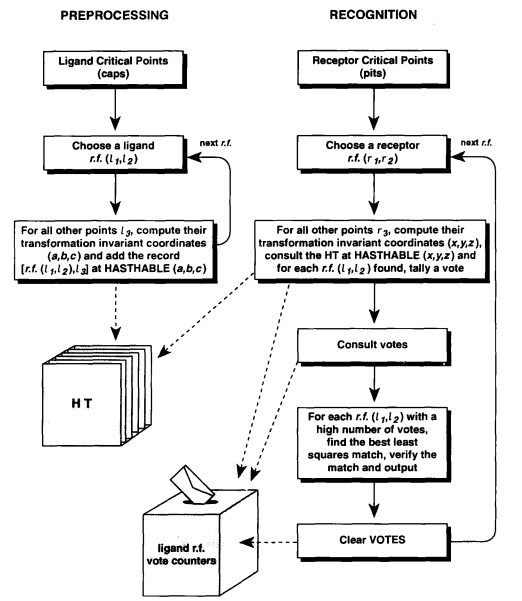
\includegraphics[width=0.5\linewidth]{geometricHashingScheme}}
  \caption{Fluxograma sobre o geometric hashing. Tirado de \cite{geometry}}
  \label{geometricFig}
\end{figure}

\subsubsection{BoGIE}
\label{bogieAlg}
Acrónimo para \textit{Boolean Geometric Interaction Evaluation}\cite{teseProf} \cite{biggerPaper}, é um método de pesquisa em grelha utilizado na primeira fase do BiGGER, que é referido no ponto \ref{biggerAlg}, mais precisamente na amostragem da população total de configurações possiveis para milhares.

 Existem dois processos principais a considerar, sendo o primeiro a definição de uma matriz tridimensional de booleanos em que cada posição da matriz representa uma parcela da forma que o complexo assume.
 
 Um nó da matriz assume valor 1, se a celula corresponde a uma parcela da proteina cujo centro se encontra a uma distancia tri-dimensional, designada por esfera de Van der Waals, de qualquer outro átomo pertencente a outra proteina, e o valor 0, se a mesma corresponder a frações do complexo que são consideradas como externas.

O segundo passo gera duas matrizes de valores booleanos semelhantes às anteriores para cada um dos elementos do par: a matriz de superficie (\textit{surface matrix}) e a matriz central (\textit{core matrix}) tal como está ilustrado graficamente na figura \ref{fig:fig2subfig}.

Os elementos celulares que ocupam a matriz de superficie são aqueles que na matriz inicial do passo anterior assumiram valor 1 mas tinham vizinhos com valor 0, ou seja, pretende-se os pontos de fronteira. 
 
 Na segunda matriz constam as células em que quer o seu valor, quer o das suas células vizinhas assumem valor verdadeiro, o que corresponde a posições em que o seu centro está próximo do centro do complexo proteico ou podendo até mesmo coincidir. 
 
 A forma de garantir que se consegue obter a superficie molecular da proteina é através da operação lógica XOR (OU exclusivo), que terá como output 1 apenas nos pontos da fronteira, pois é aqui que o resultado do XOR associado aos dois pontos selecionados dá o valor verdadeiro, já que os valores entre as duas células são diferentes e falso se forem iguais.
 
Sendo assim a complexidade deste algoritmo está associada mais com o primeiro passo do que com o segundo, já que este ltimo depende do output da matriz resultante do primeiro passo e apenas executa um conjunto de operações XOR o que não é assim tão custoso em termos de memória e tempo comparando com a medição para cada célula de uma distância.

\begin{figure}[ht]
  \centering
    {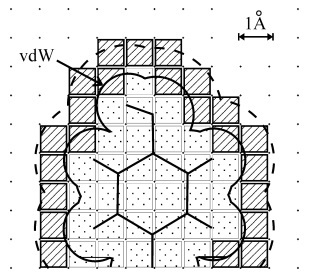
\includegraphics[width=0.5\linewidth]{figura1}}
  \caption{Representação em 2D das matrizes resultantes do segundo passo do BoGIE, as células preenchidas a tracejado diagonal correspondem à matriz de superficie, as com pontos correspondem à matriz \textit{core} e a núvem com tracejado continuo representa o corte associado à esfera de van der waals com a proteina localizada ao centro \cite{biggerPaper}.}
  \label{fig:fig2subfig}
\end{figure}

De notar, no entanto, que ambos os passos podem ser optimizados recorrendo ao GPU, no capítulo \ref{cha3} serão detalhadas possiveis abordagens à paralelização desta etapa do BiGGER, podendo trazer melhorias para além do uso do XOR.

%These simulations require only three items : initial coordinates, a potential, and algorithms for propagation. The initial coordinates can be obtained from experimental structures, or from models, or some combination thereof
%%The potential is obtained from a force field along with the coordinates
%simple; a parameterization of the energy surface of the protein. However, given the complexity of the details of protein structure, protein force fields are divided into multiple terms, built up from model-systems and transferability is assumed. Not surprisingly, given that there are many different ways to develop model-systems and to parameterize potential energy surfaces, there are many different force field models
%These two types of protein dynamics, both of which are thermodynamic in nature, changes in protein conformations, and coupled fluctuations, are the two types of dynamics that are most amenable to study by molecular dynamics simulations, and have become particularly relevant to pharmacology with the development of the concept generalized allostery [7].

%\subsubsection{Dinamica Molecular}
%\label{dm}
%Para além das técnicas de docking descritas previamente, em que se recorre à complementaridade
%de superficie do par de proteinas, existe ainda a alternativa em usar a dinâmica
%molecular. Esta técnica é adequada para situações em que é pretendido analisar a termodinamica
%e energia cinética resultantes da ligação e separação do ligando com o receptor \cite{sledz2018protein}.
%No caso das proteinas dois tipos de dinamica: mudanças de conformação e flutuação acoplada.
%Na dinamica molecular classica, a maior parte do esforço computacional é gasto a avaliar o gradiente da energia potencial respetiva às coordenadas de uma dada configuração de átomos, sendo a computação repetida para cada passo da simulação \cite{amber2013}.
%As simulações requerem as coordenadas iniciais dos átomos das moleculas, um potencial e algoritmos para propagação. As coordenadas iniciais podem ser obtidas por estruturas obtidas experimentalmente ou através de modelos. O potencial é obtido através de um campo de forças, sendo este campos de forças uma parametrização da energia da superficie da proteina. Dada a complexidade dos detalhes relacionados com a estrutura da proteina, estes campos de forças são divididos em multiplos termos. \cite{salsbury2010molecular}
%%%%%%%%%%%%%%%%%%%%%%%%%%%%%%%%%%%%%%%%%%%%%%%%%%%%%%%%%%%%%%%%%%%%%%%%%%%%%%%%%%%%%%%%%%%%%%%%%%%%%%%%%%%%%
\subsection{Ferramentas para Docking}
Antes de ser introduzido o termo GPGPU no desenvolvimento de software para docking entre proteinas, foram desenvolvidas várias ferramentas/aproximações para o estudo das interações entre proteinas. Exemplos de casos investigados incluem o BiGGER, o ZDOCK, o FTDOCK, o 3D-Dock, o GRAMM\cite{prediction} e o HADDOCK. No entanto o ZDOCK, FTDock, 3d-Dock e GRAMM são quatro exemplos de programas que usam FFTs, sendo que apenas será apresentado o ZDOCK \cite{zdock}, já que este é uma ferramenta muito referenciada em trabalhos de implementação de optimizações em GPU de programas para docking. Também é apresentado nesta subsecção o algoritmo BiGGER \cite{biggerPaper} como alternativa às aproximações que usam FFTs, pois como foi esclarecido no capitulo \ref{cap1}, é este o algoritmo que será paralelizado no decorrer da tese. Por fim o HADDOCK \cite{dominguez2003haddock} não será considerado pois esta aproximação considera a superficie das proteinas como sendo flexivel, não estando relacionado com BIGGER, que em todo o processo considera a superficie destas como rigida.
\subsubsection{BiGGER}
\label{biggerAlg}
O BiGGER\cite{biggerPaper} é um algoritmo para docking entre proteinas que considera a superficie destas como rigido, fazendo parte do software para docking Chemera.
%Este algoritmo  representa de acordo com a classificação referida no ponto \ref{classi} enquadra-se na doutrina de docking rigido.

Este algoritmo permite consiste em dois passos: o primeiro efectua uma redução de possiveis configurações resultantes de passos de translação e rotação população de cerca de $10^{15}$ configurações para uma amostra com poucos milhares de configurações corretas, através do algoritmo BoGIE relatado no ponto \ref{bogieAlg}.

A segunda fase do algoritmo consiste em aplicar metodologias de aprendizagem automática de modo a que se possa prever qual das configurações resultantes corresponde ao melhor ajuste entre os dois complexos, isto é, a que tem o score mais elevado.
 
Em termos de complexidade temporal, este algoritmo assume valores mais optimais ($O(N^{2,8})$) do que os algoritmos que recorrem ao Fast Fourier Transform. 

O motivo pelo qual das duas vertentes de algoritmos, o BiGGER assume-se com perfomance superior em termos de computação, deve-se ao facto de o BiGGER ter sido implementado com diversas optimizações face aos algoritmos FFT. 

Sendo uma das optimizações o uso de uma heurística mais eficiente no passo da eliminação de possibilidades: descarta situações em que existem sobreposições entre \textit{cores} ou até mesmo situações que não cumprem com os limites impostos nas restrições introduzidas . 

O tempo de execução do algoritmo, segundo os autores do mesmo, estava situado entre as 2H e as 8H, dependendo do par de proteinas em contraste com o tempo de execução para FTT que ronda as 6H, numa máquina com um CPU do ano de 2000 (Intel Pentium II 450 MHz dispõe apenas 1 core). 

Segundo a lei de Moore, o número de transistors presentes num CPU duplica a cada 2 anos, e por consequência a capacidade computacional, pelo que num computador em 2018 o tempo de execução do BiGGER provavelmente será menor, demorando entre 1H e 4H por exemplo.
\subsubsection{ZDOCK}
%introdução ZDOCK
O ZDOCK é um programa de docking entre pares de proteinas que usa FFT para optimizar os cálculos respetivos às caracteristicas das proteinas complementaridade de formato, electroestática e dessolvatação (desolvation), sendo este o aspeto que faz com que o ZDOCK tenha uma performance positiva. O processo de funcionamento deste algoritmo foi abordado em \cite{zdock}.
%COmo funciona
Aborda a pesquisa de combinações na primeira fase do docking através de uma grelha de pontos. Ao contrário do BiGGER, que considera a superficie e o core, o ZDOCK considera apenas os pontos circundantes ao receptor. O número total de pontos desta grelha que correspondem a pontos do ligando contribuem para uma função de score especifica chamada GSC (Grid-based Shape Complementarity), tem ainda uma subtração que consiste na penalização de confronto entre os pares de proteinas \cite{chen2002docking}. Existe ainda a função de score PSC (Pair-based Shape Complementarity) que aplica o mesmo raciocinio para o GSC, inclusive a penalização, mas apenas considera os pares de átomos receptor-ligando que se encontram a uma dada distância.
Existem quatro possibilidades para as funções de score: combinar as ditas caracteristicas químicas das proteinas (GSC + dessolvatação + eletrostatica entre o par) numa só função, usar apenas PSC, combinar está ultima com a dessolvatação e substituir a primeira alternativa referida pelo PSC. Estas combinações são consideradas pois apenas usar GSC ou PSC não garante as soluções mais precisas, pelo que é necessário existir uma função de score a complementar uma das duas. \par
%Performance
%Diferenças em relação ao BiGGER
A diferença entre esta ferramenta e o BiGGER foca-se essencialmente na complexidade temporal: o ZDOCK por recorrer a FFT, requer a mesma complexidade temporal deste, tendo o BiGGER a complexidade temporal que garante a performance superior.
No entanto, a grande diferença entre os dois foca-se no modo como é simulada o docking. O ZDOCK faz comparações entre os pontos da grelha, quer para determinar uma correspondencia, quer para comparar a distancia entre os elementos de um dado par de atomos  para determinar os valores da função de score. O BiGGER, por outro lado, apenas faz operações booleanas sobre as suas grelhas com os pontos de superficie.  

%The complete docking package, named
%FTDOCK, consists of approximately 3,500 lines of
%Fortran 77 and Perl 5.0 (Wall & Schwartz, 1991)
%code designed to run under the UNIX operating
%system
%A complete docking experiment
%including post-®ltering requires approximately
%six hours of CPU time using eight
%processors simultaneously
%The ftdock algorithm is based on that of Katchalski-Katzir [4]. It discretises the two
%molecules onto orthogonal grids and performs a global scan of translational and rotational
%space. In order to scan rotational space it is necessary to rediscretise one of the molecules
%(for speed the smaller) for each rotation. The scoring method is primarily a surface complementarity
%score between the two grids, and this is shown in Figure 2. To speed up the surface
%complementarity calculations, which are convolutions of two grids, Fourier Transforms are
%used. This means that the convolutions are replaced with multiplications in Fourier space,
%and despite having to perform the forward and reverse Fourier Transforms, this decreases
%the overall computation required. The surface complementarity was the only score used in
%the original method. The original work on ftdock by Gabb [2] found it a useful addition to
%include an electrostatic filter, and this is again implemented in the current version (though
%it can be turned off).
%The additional constraint of removing predictions
%with unfavourable electrostatic interactions
%markedly improves the ranking of correctly docked
%structures in the global search
%\subsubsection{FTDock}
%Esta ferramenta foi implementada em Perl e Fortran, apenas disponivel para sistemas operativos UNIX \cite{ftdock}.
%Em termos de docking, usa a complementaridade de formato e eletroestática como função de score assim como a técnica de correlação de matrizes por FFT descrita no ponto \ref{fft}, sendo uma ferramenta semelhante ao ZDOCK. No entanto para o FTDock desenvolveram-se melhorias em relação à versão do FFT introduzida em 1992. É considerado na função de score sobre a eletroestatica do par um constrangimento adicional, de forma a aumentar a precisão do algoritmo na fase de pesquisa global.
%O tempo de execução para um docking completo (são completadas as duas fases) demorava seis horas para oito processadores em simultaneo. 
%%%%%%%%%%%%%%%%%%%%%%%%%%%%%%%%%%%%%%%%%%%%%%%%%%%%%%%%%%%%%%%%%%%%%%%%%%%%%%%%%%%%%%%%%%%%%%%%%%%%%%%%%%%%%%%%%%%%%%%%
%secção GPU
%GPGPU stands for General-Purpose computation on Graphics Processing Units, also known as GPU Computing. Graphics Processing Units (GPUs) are high-performance many-core processors capable of very high computation and data throughput.  Once specially designed for computer graphics and difficult to program, today’s GPUs are general-purpose parallel processors with support for accessible programming interfaces and industry-standard languages such as C.  Developers who port their applications to GPUs often achieve speedups of orders of magnitude vs. optimized CPU implementations. The goal of GPGPU.org is to catalog the current and historical use of GPUs for general-purpose computation, and to provide a central resource for GPGPU software developers.
\section{O GPU}
\label{gpus}

\subsection{Arquitectura e Modelo de Execução}
\label{gpuArch}
Tal como os CPUs, os GPUs também seguem uma arquitetura. Os conceitos essenciais das arquitecturas dos GPUs modernos são transversais aos diferentes modelos existentes, inclusive de diferentes marcas. No presente documento serão utilizadas como referência as arquitecturas dos GPUs NVIDIA, em particular a arquitetura mais recente ( em 2018) de nome Volta\cite{voltaArch} que está presente nos GPUs de modelo Tesla V100 (figura \ref{voltaArch}). Esta nova arquitetura traz diversas optimizações de hardware e lógicas face às versões anteriores, eg. Pascal, Maxwel e Kepler, para desempenho em computações na área do deep learning. Também é uma arquitetura própria para acelerações relacionadas com aplicações que usam data-centers.


Em termos gerais as arquiteturas têm os seguintes elementos:
\begin{itemize}
\item \textbf{Streaming Multiprocessors} : Cada GPU tem uma quantidade variável de \textit{streaming multi-processors} (SMs). Os SMs, por seu lado, são compostos por um conjunto de processadores escalares (SPs) que são também conhecidos como os \textit{cores} do GPU. Os SMs Assumem a função de executar os \textit{kernels} (sobre estes últimos é feita uma descrição detalhada na subsecção \ref{exec}). Têm ciclos de relógio mais baixos, mas suportam paralelismo ao nível de instrução. As componentes dos SMs vão sendo melhoradas face aos SMs de arquiteturas anteriores. A destacar o número de registos que os SMs vão dispondo, a cache L1 e o número de \textit{cores} de execução \cite{wilt_2013}.Os SMs são agrupados em partições de hardware com tamanho igual denominados GPU processing clusters (GPCs) e o número de GPCs presentes num GPU depende da arquitetura.  \par
Na arquitetura Volta, cada um dos 84 SMs presentes, estão particionados em quatro blocos de processamento como se pode ver na figura \ref{voltaSM}. Cada um destes blocos é composto por 16 cores FP32, 8 cores FP64 e 16 cores INT32. Cada SM é capaz de executar no máximo 2048 threads. Foram aplicadas optimizações nos SMs para a versão Volta face a versões anteriores, mais precisamente a adição de \textit{tensor cores}, que são componentes especiais para acelerar as operações associadas a redes neuronais. O GV100 encontra-se dividido em 6 GPCs, cada um destes GPCs contem 14 SMs.
 \begin{figure}[ht]
  \centering
    {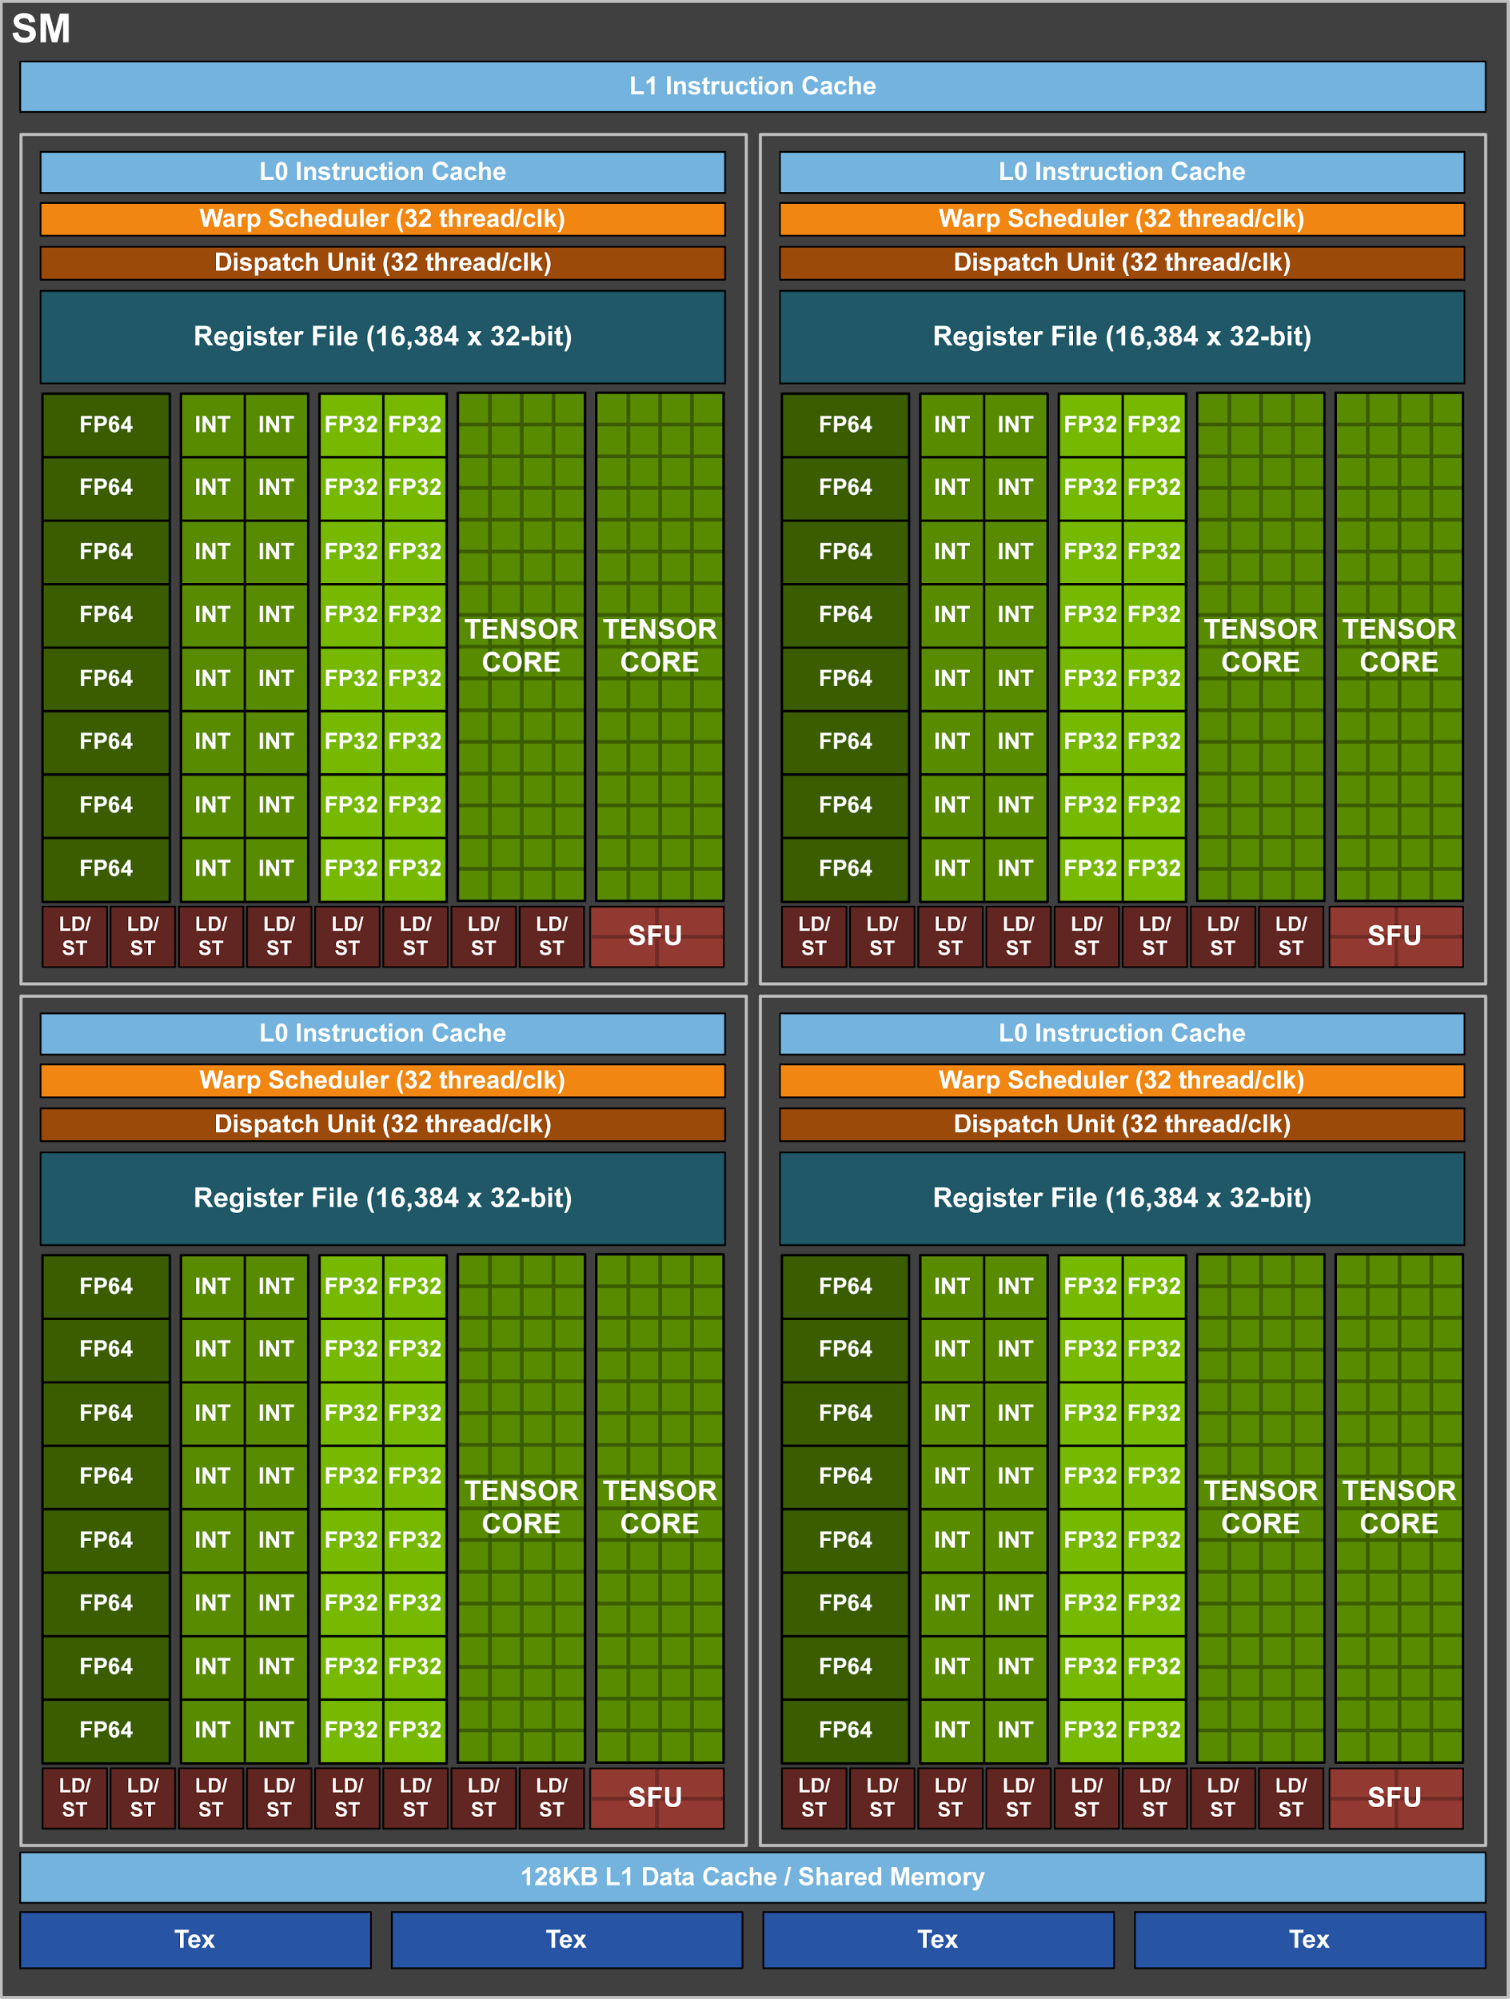
\includegraphics[width=0.55\linewidth]{voltaSM.png}}
  \caption{Esquema do SM para o GV100\cite{voltaArch}.}
  \label{voltaSM}
 \end{figure}
% Hierarquia de memória: O GPU contém uma memória global, partilhada por todos os SMs. (tamanhos?)
%
%Além disso, existem ainda dois níveis …
\item \textbf{Hierarquia de memória}: O GPU contém uma memória global, partilhada por todos os SMs. Esta memória global tem um quantidade de espaço que varia entre 12GB para a arquitetura Kepler e 16GB para a arquitetura Volta.  Além disso, existem ainda dois níveis de cache a considerar. As caches L1 são usadas para melhorar a latência das operações globais de escrita e leitura e como especificado no ponto anterior, estas fazem parte dos SMs. Existe ainda uma cache partilhada L2 para complementar a presença das L1. A cache L2 é uma cache de escrita/leitura com uma politica de substituição \textit{write-back}. Esta cache responde a pedidos de instruções load, store assim como instruções atómicas de ambos SM e respetivas caches L1, preenchendo de forma igual as respetivas caches \cite{nickolls2010gpu}. A partir da arquitetura Volta a cache L1 e a memória partilhada de cada SM passam a estar juntas, o que traz beneficios para a L1 como o aumento da capacidade de memória/SM em 7 vezes a capacidade da arquitetura Pascal, a diminuição da latência de acesso e o aumento da banda-larga\cite{voltaArch}.  Também existirá uma nova cache de instruções L0 em cada um dos blocos do GV100, melhorando a eficiência face ao uso de buffers de instruções dos SMs anteriores. 
\end{itemize}
  \begin{figure}[ht]
  \centering
    {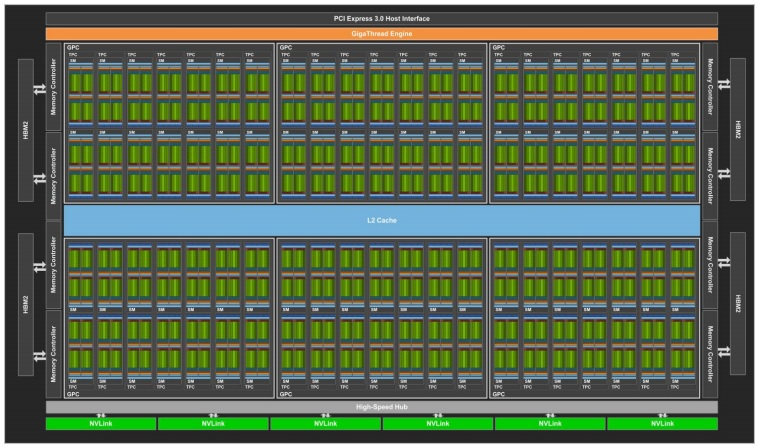
\includegraphics[width=1\linewidth]{archVolta}}
  \caption{Esquema da arquitetura do GPU, mais precisamente do Volta GV100\cite{voltaArch}. Esta é a arquitetura mais recente que NVIDIA lançou no mercado.}
  \label{voltaArch}
\end{figure}
\subsubsection{Capacidade de computação de uma arquitetura}
Todas as arquiteturas NVIDIA têm o conceito de capacidade de computação rótulado a um valor (tabela \ref{tabelaCap}). Este valor determina as funcionalidades permitidas pelo hardware respetivo, assim como as melhorias nas componentes de hardware face a arquiteturas anteriores. O número de registos presentes no GPU, o número máximo de threads em cada SM e a granularidade de alocação dos registos variam com as diferentes capacidades de computação \cite{cudaProgGuide}. O valor da capacidade de computação pode ser usado pelas aplicações em tempo de execução para determinar o que o GPU presente na máquina dispõe em termos de funcionalidades e instruções nativas. Este valor é também décimal, sendo a casa das unidades respetiva ao número de revisão maior e o das décimas ao número de revisão menor. Se uma arquitetura tem um valor de capacidade de computação superior a uma segunda, por ser mais recente, quer dizer a primeira arquitetura tem as funcionalidades e caracteristicas de hardware da segunda, com mais umas adições novas, assim como a primeira consegue resolver os problemas endereçados na segunda. O que faz com que um programa que tenha sido implementado em referência a uma arquitetura Kepler, com capacidade computacional 3.5, possa ser compativel para execução num GPU com a arquitetura Volta, com capacidade computacional 7.0.
\begin{table}[]
\centering

\begin{tabular}{|l|l|l|l|l|}
\hline
GPU             & Kepler GK180 & Maxwell GM200 & Pascal GP100 & Volta GV100 \\ \hline
Cap. Computação & 3.5          & 5.2           & 6.0          & 7.0         \\ \hline
\end{tabular}
\caption{Tabela de capacidades computacionais das arquiteturas NVIDIA mais recentes. Adaptado de \cite{voltaArch}.}
\label{tabelaCap}
\end{table}
%Modelo de execução
%eu trocava a ordem deste dois parágrafos
%
%primeiro dizes como é que computação é estrutura e depois como é que é executada
%
%Neste segundo ponto, tens de tornar claro que um bloco é executado por um SM e que um SM pode executar vários blocos (desde que tenha recursos hardware para tal). Depois disso podes entrar na discussão como é que os blocos são executados pelo SM. A tal divisão em warps
\subsubsection{Modelo de execução}
\label{exec}
  %          papel do host e do device
O modelo de execução em GPU inclui o conceito de computação heterógenea, em que temos dois conjuntos de computações de carácter geral no GPU concorrentes a executar código: o conjunto \textit{host} composto por CPUs e o \textit{device}, composto por GPUs. Os dois sistemas desempenham papeis diferentes. O \textit{host} coordena as transferências de dados a manipular entre as duas entidades e a invocação dos \textit{kernels}. Também gera a alocação de memória nos \textit{devices}.
%kernel 
Os \textit{kernels} são funções programadas para executar um determinado número de vezes $N$ em paralelo por $N$ threads do GPU, tendo cada uma destas threads um ID único, que é acessível dentro do \textit{kernel}. O  executa os \textit{kernels} e manipula os dados que o \textit{host} alocou e transmitiu, retornando o resultado para o \textit{host}.
%Threads\cite{cudaProgGuide}
% Warps
% A execução dos blocos em warps pelos SMs
 As  \textit{threads} do GPU são consideradas como \textit{lightweight} pois são escalonadas em grupos conhecidos como \textit{warps}\cite{cudaProgGuide}\footnote[1] {Tendo em conta a quantidade de  \textit{threads} individuais que têm de ser geridas e executadas de forma eficiente, é empregado pelos SMs uma arquitetura especifica para o efeito, denominada SIMT (\textit{Single-Instruction Multiple-Thread}) \cite{nvidiaTesla}.
É ainda permitido por parte de qualquer uma das arquiteturas referidas a criação, gestão, escalonamento e execução de  \textit{threads} concurrentes em grupos de 32 cada. Estes grupos denominam-se \textit{warps}, podendo cada bloco de  \textit{threads} do CUDA ter 1 ou mais warps
\cite{nickolls2010gpu}.}. No caso do GPU ter de ficar à espera de um desses grupos, este tem a possibilidade de avançar para outro, pelo que não é necessário haver o sistema de trocas presente no CPU. As \textit{cores} do CPU minimizam a latência para um número muito reduzido de threads de cada vez, enquanto que as \textit{cores} do GPU permitem a este gerir um número muito maior de threads mais ligeiras, maximizando o \textit{throughput}.
     %       a estruturação da computação em grelha, bloco     
  \begin{figure}[ht]
  \centering
    {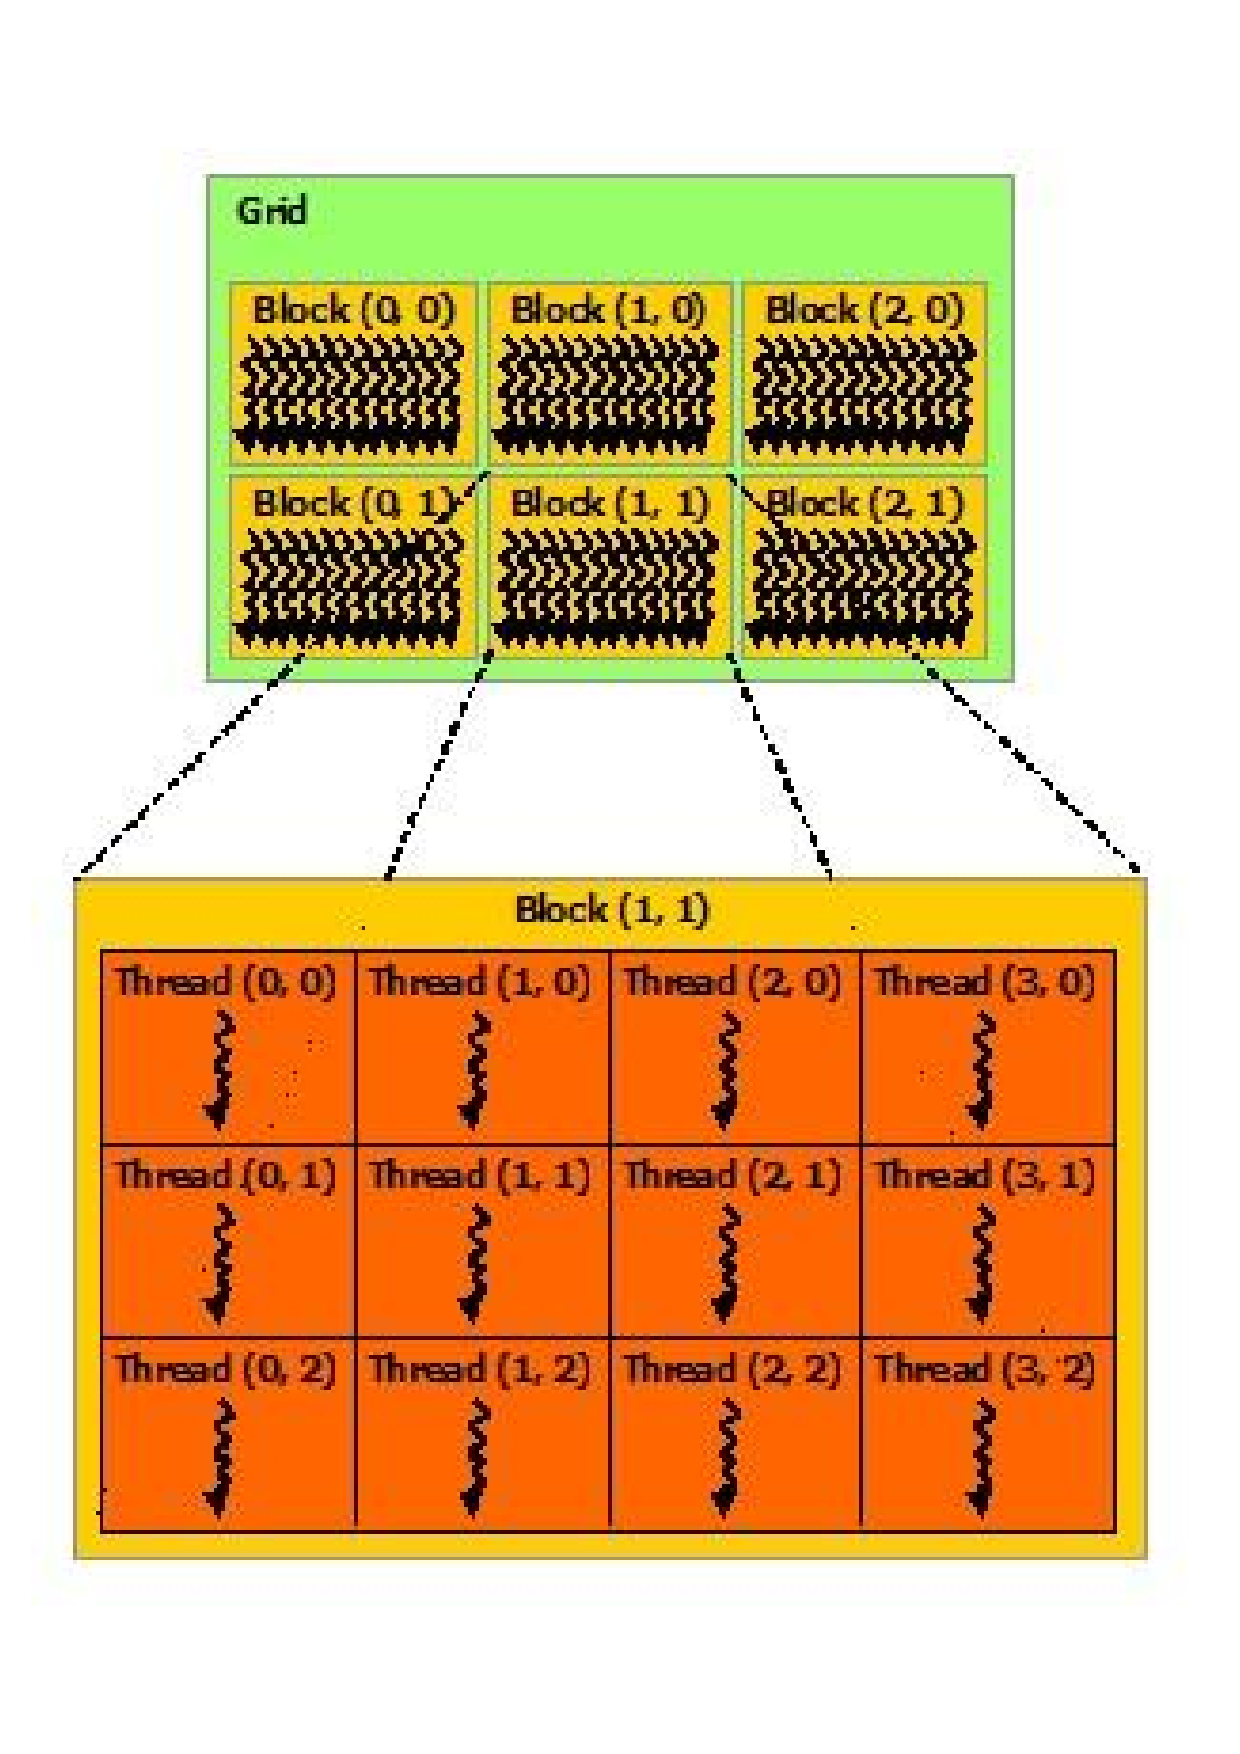
\includegraphics[width=0.5\linewidth]{threadGrid.pdf}}
  \caption{Ilustração de uma grelha de threadblocks, detalhando um elemento da grelha para ilustrar os pormenores de um bloco de threads. Neste caso o bloco é bi-dimensional, mas existe a possiblidade de ser tri-dimensional, o mesmo se aplica à grelha \cite{cpg}.}
  \label{threadGrid}
\end{figure}
     %Thread block
Uma computação que é executada pelo GPU tem de ser estruturada numa grelha. \par Cada um dos elementos da grelha é um bloco referido como \textit{thread block} (na figura \ref{threadGrid} podemos consultar um exemplo de um \textit{thread block}). A dimensão máxima associada ao tamanho de um \textit{thread block} é dependente da arquitetura. No caso das arquiteturas mais recentes é 1024 threads. Numa situação em que é pretendido fazer computações numa estrutura de dados de tamanho superior a 1024 unidades, a mesma é repartida em partes de tamanho igual, sendo cada uma das partes é atribuida a um \textit{thread block} para processamento. 
 
\subsection{Modelos Base de Programação} 
\label{progGPU}
%  CUDA e OpenCL
Em termos de programação em GPUs existem como APIs o CUDA (\textit{Compute Unified Device Architecture})\cite{cudaZone} que foi implementado pela NVIDIA e o OpenCL(\textit{Open computing language})\cite{openCL}. Ambos suportam a linguagem C/C++ apesar de poderem suportar outras linguagens, como por exemplo Free Pascal no caso do OpenCL. O CUDA apenas funciona com placas da NVIDIA enquanto que o OpenCL permite efectuar paralelizações em hardware de diferentes arquiteturas e tipos, desde CPUs a \textit{clusters}. Sobre o CUDA existem bindings para outras linguagens, como por exemplo pyCUDA para a linguagem Python ou a biblioteca especializada com o cuFFT\cite{nvidiaFFT} para acelerar a técnica FFT.  \cite{openclProf}

%       o que é que o programador tem de expressar 
%o código que cada thread da grelha deve executar
%O que é que o programador deve elaborar para que o programa funcione -  não interessam o pormenores de sintaxe  
 O programador deve elaborar código em duas vertentes. Por um lado tem de programar as tarefas do lado do \textit{host}, mais precisamente alocações de memória no GPU, eventuais transferências de dados entre o CPU e o GPU que vão ser manipulados na execução dos \textit{kernels} e quando é que os estes são invocados. Sobre os \textit{kernels} o programador tem ainda de especificar os parametros de execução (dimensão do bloco e número de threads a invocar no \textit{kernel}), sendo que com estes parametros o CUDA/OpenCL determina a quantidade de threads a lançar. Por outro tem de implementar o código que cada thread da grelha deve executar, a correr dentro do \textit{kernel} em que pretende fazer a respetiva paralelização. O código sequêncial deve ser executado no \textit{host} e o código a paralelizar no programa deve ser executado no \textit{device}.

%thread blocks e sincronização
%Sobre CUDA, é permitido pela API a sincronização de threads dentro de um thread block, no entanto a sincronização entre thread blocks através do uso da chamada referida não é possivel, já que estes são independentes entre si. No entanto, em versões mais recentes, tornou-se possivel a sincronização neste ultimo caso utlizando instruções e primitivas especificas suportadas pelo respetivo hardware CUDA. Uma alternativa para sincronizar blocos de threads é garantir que o kernel é terminado.


\subsection{Optimizações}
\label{optmi}
%%%%%%
Um dos passos na programação de versões aceleradas em GPU para um programa consiste em aplicar um conjunto de possiveis optimizações à versão paralelizada do programa, de forma a optimizar a performance do programa para que se possa comparar o resultado final com as expetativas iniciais.
Existem quatros aspetos a considerar quando pretendemos optimizar um programa recorrendo ao GPU, com os respetivos detalhes de acordo com \cite{cudaProgGuide}:
\begin{itemize}
%        entre o host e o GPU - sobreposição dec computação com comunicação 
%A stream in CUDA is a sequence of operations that execute on the device in the order in which they are issued by the host code. While operations within a stream are guaranteed to execute in the prescribed order, operations in different streams can be interleaved and, when possible, they can even run concurrently
\item{\textbf{Sobreposição de comunicação com computação}} : 
É necessário sobrepor as computações do \textit{host} e do device com a comunicação pois ter as duas sem sobreposição pode afectar a performance. Em CUDA tal pode ser feito através de \textit{streams}. \textit{Streams} são sequências de operações que são executadas no \textit{device}, por uma dada ordem imposta pelo \textit{host}  podendo ser cópias de memória ou execuções de \textit{kernels}. Apesar das operações numa \textit{stream} terem de ser executadas pela ordem imposta pelo \textit{host}, as operações entre \textit{streams} podem ser interligadas, havendo sobreposição, e por consequência, possível a esconder a latência associada à transferência de dados entre o \textit{host} e o \textit{device}. Dependendo da arquitetura do device, é possivel sobrepor a comunicação entre host e \textit{device} e a computação respetiva à execução do \textit{kernels}. O requisito é ambas as instruções serem de \textit{streams} diferentes e não por omissão\footnote[2]{Uma \textit{stream} por omissão tem o seu \textit{streamID} com o valor nulo. Pelo que o pretendido é uma \textit{stream} cujo o seu id seja diferente de 0. }, caso contrário as instruções terão de ficar à espera de instruções anteriores no device terem acabado, sem poderem começar, o que  impossibilita a sobreposição das instruções e esconder a latência de comunicação.

%      ocupação do GPU
\item{\textbf{Taxa de ocupação do GPU}} :
É essencial, para a performance ser optimal, manter os SMs do GPU o mais ocupados possivel no decorrer da execução da aplicação, devendo existir uma distribuição de trabalho equilibrada entre os SMs. A aplicação final deve estar implementada de forma a que use os threads e respetivos blocos maximizando a utilização do hardware, evitando situações em que se deixa de impor a distribuição livre de trabalho entre os SMs.
A taxa de ocupação determina o quão efectivamente o GPU se encontra ocupado, isto é, o número de \textit{warps} que estão activos em relação ao número máximo de \textit{warps} que o GPU consegue activar. É pretendido que esteja o mais próximo possível de um certo limite que depende da capacidade de computação da arquitetura do GPU \footnote[3]{Como foi descrito no ponto \ref{gpuArch}, a respeito da capacidade de computação de uma arquitetura, o respetivo valor está associado ao número de registos presentes em cada SM, que pode variar dependendo do valor da capacidade.}. Exceder este limite não traz melhorias de performance, no entanto se o código estiver longe de atingir este limite é garantido que a performance não vai ser optimal. Para garantir a taxa de ocupação adequada ao GPU, é possivel optar por garantir que os \textit{kernels} são executados ao mesmo tempo, o que é chamado de execução concorrente de \textit{kernels}. 

%        acesso a memória global e partilhada aqui tens de falar é dos acessos coalescentes à memória global e na utilização da memória partilhada
%Global memory resides in device memory and device memory is accessed via 32-, 64-, or 128-byte memory transactions. These memory transactions must be naturally aligned: Only the 32-, 64-, or 128-byte segments of device memory that are aligned to their size (i.e., whose first address is a multiple of their size) can be read or written by memory transactions.
%
%When a warp executes an instruction that accesses global memory, it coalesces the memory accesses of the threads within the warp into one or more of these memory transactions depending on the size of the word accessed by each thread and the distribution of the memory addresses across the threads. In general, the more transactions are necessary, the more unused words are transferred in addition to the words accessed by the threads, reducing the instruction throughput accordingly.
% How many transactions are necessary and how much throughput is ultimately affected varies with the compute capability of the device
%Grouping of threads into warps is not only relevant to computation, but also to global memory accesses. The device coalesces global memory loads and stores issued by threads of a warp into as few transactions as possible to minimize DRAM bandwidth
%Agrupar as threads em warps é relevante para os acessos à memória global. O device coalesce os loads e stores à memoria global na menor quantidade de transações possiveis para minimizar \cite{}
%
%Because it is on-chip, shared memory has much higher bandwidth and much lower latency than local or global memory.
%
%To achieve high bandwidth, shared memory is divided into equally-sized memory modules, called banks, which can be accessed simultaneously. Any memory read or write request made of n addresses that fall in n distinct memory banks can therefore be serviced simultaneously, yielding an overall bandwidth that is n times as high as the bandwidth of a single module.
%
%However, if two addresses of a memory request fall in the same memory bank, there is a bank conflict and the access has to be serialized. The hardware splits a memory request with bank conflicts into as many separate conflict-free requests as necessary, decreasing throughput by a factor equal to the number of separate memory requests. If the number of separate memory requests is n, the initial memory request is said to cause n-way bank conflicts.

\item {\textbf{Optimizações de memória}} : Em que são consideradas as memórias global e partilhada do device.
Sobre a memória global, esta é acessivel via transações de memória de 32, 64 ou 128 bytes. Estas transações devem estar naturalmente alinhadas, o que implica apenas os segmentos de memória cujo primeiro endereço é um multiplo do tamanho do segmento, sendo este 32, 64 ou 128 bytes poderem ser escritos ou lidos pelas transações.
 Quando um warp executa uma instrução que pretende aceder à memória global, é feita a coalescência dos acessos à memoria por parte das threads do warp numa quantidade de transações de memória que depende do tamanho da palavra acedida por cada thread e da distribuição dos endereços de memória pelas threads do warp. Quanto maior é o número de transações necessárias, maior é o número de palavras não usadas que são transferidos em adição às palavras acedidas pelas threads, o que tem como efeito a redução do \textit{throughput} de instruções\cite{cpg}. \par

No caso da memória partilhada, esta tem uma latência de acessos menor do que a memória global, e largura de banda superior. A memória partilhada está dividia em módulos de memória com tamanho igual, chamados \textit{banks}. Os \textit{banks} podem ser acedidos de forma simultânea. Existe a possibilidade de ocorrer \textit{bank conflicts} quando dois endereços de um pedido de acesso à memória correspondem ao mesmo \textit{bank}.  Tendo o acesso de ser serializado e o pedido dividido em sub-pedidos separados que são livres de conflito. Por consequência o throughput é reduzido em um factor que depende do número de divisões efectuadas.

%        evitar escolhas — divergência nos warps
\item{\textbf{Controlo de fluxos}} : É muito importante evitar que ocorram divergências na execução de threads de um mesmo \textit{warp}. Esta situação pode acontecer quando dentro do código de um \textit{kernel} existem instruções de controlo de fluxos (eg. if, switch,while, do while e for) o que leva à redução do throughput de instruções devido ao facto de existirem threads dentro de um \textit{warp} a divergir em caminhos de execução diferentes. No entanto podem existir situações em que o fluxo de controlo depende unicamente do thread ID, nessas situações é importante a escrita da condição de controlo de forma a atenuar o número de \textit{warps} a divergir. Outra forma de garantir que não existem divergências é tornar fácil para o compilador \footnote[4]{ No caso do CUDA o compilador é o NVCC, no caso do OpenCL é o OpenCL Compiler.} o uso de \textit{branch predication} ou seja, o compilador desenrola os loops/condições impedindo divergências de \textit{warps}. Apenas as instruções em que o predicado assume o valor verdadeiro em relação à condição de controlo são executadas.
\end{itemize}
%%%%%%


%%%%%%%%%%%%%%%%%%%%%%%%%%%%%%%%%%%%%%%%%%%%%%%%%%%%%%%%%%%%%%%%%%%%%%%%%%%%%%%%%%%%%%%%%%%%%%%%%%%%%%%%%%%%%%%%%%%%%%%%

%Existem vários trabalhos que endereçam a paralelização de étpadas de … no GPU […..] (todos os que encontraste, mesmo que não os apresentes). Destes, nesta secção iremos apresentar o ...., o… 
\section{Docking em GPU}
\label{gpus1}
Existem vários trabalhos que focam a paralelização de etapas constituintes do processo de docking no GPU\footnote[5]{Na investigação foram encontrados como programas de docking que podem ser executados em GPU o Megadock, o PIPER, o HEX, o AutoDock e o MolDock. Estes dois ultimos são para docking entre proteina-ligando.}. Destes, são abordados nesta secção o Megadock, o PIPER e o AutoDock. O Megadock e o PIPER são os programas mais conhecidos cujo funcionamento é semelhante ao do BiGGER. O AutoDock, apesar de ser um programa cujo funcionamento é diferente do BiGGER, foi considerado pois foi desenvolvida uma paralelização à etapa de \textit{scoring} \cite{autodockCuda} onde são discutidas duas abordagens em função da taxa de ocupação do GPU assim como é discutida a possibilidade sobre o uso da memória partilhada deste. O Megadock é um dos programas em que a aceleração aumentou drásticamente após o desenvolvimento da versão 4.0, demonstrando os beneficios de adaptar um programa para executar em GPU. Os trabalhos sobre o Megadock \cite{shimoda2015protein} \cite{megadock40} abordam uma possibilidade para mapear etapas do funcionamento do BiGGER para o GPU.\par Foi considerado o PIPER pois em termos históricos este foi um dos primeiros programas para docking a ser acelerado usando o CUDA\cite{piper2009gpu}. A subsecção respetiva mostra ainda a importância de aplicar manutenção ao código acelerado de versões anteriores e o impacto da não aplicação de manutenções na performance quando se executa um programa com hardware mais recente, sendo desenvolvida uma versão mais recente \cite{piper2014gpu}.
%Um aspeto comum entre todos é terem uma versão de software alternativo que funciona na web, ou seja, têm um web-server, que oferece os serviços que o programa original dispõe. A execução não é feita na máquina local mas sim numa repartição de clusters.
%Já existem vários softwares e artigos dedicados à introdução de paralelizações ao FFT \cite{ritchiew} o que muitos têm em comum é o facto de utilizarem CUDA, neste caso utilizam CuFFT. 
%Pending a correlação de matrizes é paralelizada no FFT?
%O CuFFT é uma versão própria do CUDA que fornece as implementações necessárias para que a perfomance do algoritmo seja aumentada em 10x, face às versões que utilizam o CPU para o processamento respetivo\cite{nvidiaFFT} . 

\subsection {Megadock}
\label{megaD}
%Introcução megadock
O Megadock 4.0\cite{megadock40} é um software de protein-protein docking de origem japonesa, com optimizações para executar recorrendo ao GPU. Este programa usa a técnica de Fast Fourier Transform na sua correlação de matrizes.

Este programa é adequado para máquinas que têm muitos \textit{cores} de GPU e CPU à disposição, caracteristicas tipicas de supercomputadores. No entanto é possivel utilizar o megadock em computadores pessoais, alterando a flag de compilação do programa para usar apenas a implementação GPU.
%detalhes implementação Sistema geral, clustering 
O funcionamento do Megadock 4.0 envolve a criação de um processo master que faz a aquisição de uma lista de pares de proteinas e distribui o docking dos pares para os workers presentes nos nós disponiveis.
 Estes, por sua vez, distribuem o trabalho de calcular a rotação do ligando em cada nó da lista, pelos diversos GPUs e CPUs do nó do cluster. A execução pelos GPUs de cada nó é feita por CUDA e pelos CPUs por OpenMP . 
 %vantagens 
 Uma das vantagens que este protocolo assume é a tolerância a falhas pois o nó master consegue supervisionar os resultados dos jobs executados pelos workers, além disso é escalável com o número de elementos que compõem o cluster.

   \begin{figure}[ht]
  \centering
    {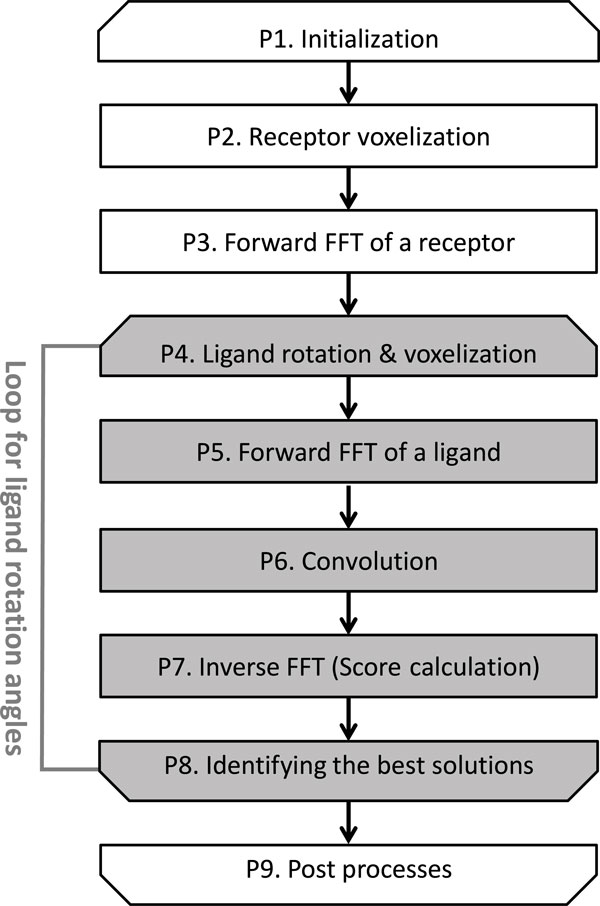
\includegraphics[width=0.5\linewidth]{MegadockGPU}}
  \caption{Etapas do processo de docking no Megadock. As etapas a cinzento foram aceleradas por GPU\cite{shimoda2015protein}. }
  \label{megadockGPU}
\end{figure}
 \subsubsection{Execução em GPUs}
 %Referir o que é implementado para cuda no megadock e em que medida é importante para o BIGGER : O que é que os GPUs fazem
As acelerações implementadas para o Megadock consistem em optimizações para 6 etapas. Na figura \ref{megadockGPU} ilustram-se as etapas no processo de docking no Megadock, foi aplicado um profile sobre o funcionamento do programa com apenas 1 core do CPU, registando os tempos de execução em cada etapa. Os resultados presentes em \cite{shimoda2015protein} indicam que as etapas P4 a P8 consomem a maioria do tempo de execução. Estas etapas constituem um ciclo em que se iteram as possibilidades de ângulos para a rotação do ligando. No caso da P4 as coordenandas do ligando são atualizadas de acordo com uma dada matriz de rotação e o processo respetivo é independente para cada átomo, sendo paralelizável. Esta etapa foi acelerada mapeando as coordenadas atómicas do ligando para o GPU. 
A segunda vertente da P4 consiste na voxelização do ligando, em que é feita uma afectação a uma posição da grelha em relação às coordenadas atómicas de um dado átomo do ligando. As coordenadas devem pertencer à região interna da curva de van der Waals. Este processo é também paralelizável em relação a cada átomo. Pelo que nesta vertente os átomos também são processados em paralelo e mapeados para o GPU, sendo cada átomo designado a uma \textit{core} do GPU.\par Para as etapas P5 e P7, em que é feita a FFT discreta do ligando e o cálculo da inversa do FFT deste, respetivamente, foi utilizada a biblioteca especializada para FFT, cuFFT. Na etapa P6, convolução, foi aplicado um mapeamento para o GPU. E na última etapa do ciclo, P8, em que os resultados têm uma dada pontuação, foi aplicada uma operação de redução no GPU. 
Sobre a comunicação \textit{host-device}, é referido que apenas aconteceu uma vez a transferência de dados. O conteúdo da transferência inclui as coordenadas atómicas do ligando e a grelha do receptor com o FFT aplicado. \par
 %Resultados e tempos de execução
% Em termos de performance e tempos de execução, os testes efectuados em 2014 revelam que a implementação MIC do Megadock foi capaz de determinar em minutos um caso de teste que o ZDOCK determinou em duas horas.  Os resultados referidos foram obtidos por execução no supercomputador disponível no Instituto de Tecnologia de Tóquio, TSUBAME 2.0.Ficou demonstrado 420 nós, tendo cada um dos nós dois Intel Xeon X5670 e três GPUs NVIDIA Tesla K20X (GK110).
% A dimensão amostral consiste no número total de combinações de estruturas receptoras  e no número total de combinações para estruturas ligandas. No caso do Megadock 4.0, o valor a considerar para o tempo de cálculo ronda as 3H num cenário em que  5.71h para meio milhão de jobs e 11.51H para 1 milhão de jobs. Para este último teste foi utilizado a versão 2.3 do TSUBAME\cite{megadock40}. 
Em termos de performance e tempos de execução, os testes efectuados em 2014 revelam que a implementação MIC do Megadock 4.0 foi capaz de fazer em 3H, usando 420 nós, um caso de teste que requer 250.000 \textit{dockings} que versões anteriores do Megadock levariam dias \cite{megadock40}. A implementação GPU demonstrou ser 15.1 vezes mais rápida do que a versão que apenas usava um \textit{core} do CPU.
%To map a docking calculation onto a GPU, we had to write several CUDA kernel functions, which describe the processes executed on the GPU, as well as adding statements to facilitate data transfer between the host and the accelerator. We had to add the code with approximately 1,000 lines to the MEGADOCK original code with approximately 7,000 lines. Therefore, the implementation costs were high, although we were familiar with CUDA programming. Furthermore, the source code management costs were increased because the code required many branches and additional source code files for GPU computing.
\subsubsection{Conclusões}
Sobre a implementação GPU do Megadock, em que foi usado CUDA, existem aspetos que podem ser aproveitados para ajudar na paralelização do BiGGER. Os mecanismos master-worker não são tão importantes pois o trabalho a desenvolver na elaboração da dissertação não engloba programação em clusters. Ainda sobre \cite{shimoda2015protein} é revelado que a implementação MIC, apesar de ter menos custos de implementação, não é tão eficiente como a implementação GPU na aceleração do FFT . As abstrações usadas na implementação dos \textit{kernels}, no entanto, podem ser aproveitadas, mais precisamente a aplicação de uma operação de redução no passo do BiGGER que determina o ângulo de rotação optimal para o ligando. Também podem ser aproveitados os mapeamentos para o GPU descritos. Sobre os custos de implementação, é referido em \cite{shimoda2015protein} que no processo de mapear o docking para o GPU, foi necessário escrever várias funções\textit{ kernel}, assim como escrever instruções para facilitar a transferencia de dados entre o \textit{host} e o \textit{device}. No total foram acrescentadas 1000 linhas de código às 7000 que o Megadock tinha originalmente, sendo necessário adicionar ficheiros de código-fonte e ramificações no código. Pelo que é esperado que desenvolver a paralelização do BiGGER mapeando etapas do mesmo para o GPU tenha um nível similar de custos de implementação. 

%PIPER's primary advance is the use of desolvation energies in the evaluation function, in addition to the previously used shape and electrostatics terms. The desolvation terms are generated as pairwise potential terms. The PIPER algorithm proposed that by using eigenvalue-eigenvector decomposition, the number of terms needed could be limited to the P largest eigenvalues, where 2 ≤ P ≤ 4, limiting the added number of Fourier transforms to 2 to 4 forward transforms and one reverse. When GPU PIPER09 was designed, it was under the assumption that up to 18 of these desolvation terms may still be used [16]. Since then, however, it has been found that in practice only 4 terms are typically ever used; this is a key to one of the optimizations in the current work.

%Most significant is the difference in proportion of time spend on the correlation step. On the GPU, the proportion is actually even smaller than shown: the correlation time is completely hidden by the data transfer time.
%Algorithmic and usage changes in PIPER have changed the proportion of the time spent on filtering. It has been reduced in the CPU version but increased in the GPU version

%Thus the goal of optimizing the GPU filtering kernel has changed from attempting to find the top score for all coefficient sets simultaneously, to quickly finding the top score for a single coefficient set and then repeating the process.
%


%GPU PIPER09 uses a scoring and filtering kernel that finds the top scores for a rotation for all provided scoring coefficients at the same time. This method works the best when the maximum number of coefficient sets are provided at the same time, typically up to 8. In this case, the top score for each set of coefficients is calculated by a single SM. With 8 coefficient sets, 8 SMs are simultaneously occupied. 
%PIPER use has also changed. Most docking runs now use only a single coefficient set, meaning only a single SM is used. Thus the goal of optimizing the GPU filtering kernel has changed from attempting to find the top score for all coefficient sets simultaneously, to quickly finding the top score for a single coefficient set and then repeating the process.
%%Filtering and scoring on the GPU now uses two kernels which are then repeated for every set of coefficients, as well as being repeated for the number of top scores desired by the user for each coefficient set. The two kernels partition the work into two stages so that the shared memory on the GPU is used for fast memory access, and so that work is distributed across all SMs.
%In the first kernel the output data, which is the size of the molecular grid volume, or equivalently the FFT size, is partitioned among all available SMs. This is done by launching the kernel with a sufficiently large number of blocks such that every SM has a suitable quantity of work. For reasons that will be explained later, the number of blocks must be a power of two.

%non-correlation steps: filtering, grid assignment, and data transfer
%multiple sets of coefficients can be provided so that PIPER returns the top scores for each set of coefficients. PIPER is capable of returning the top N scores for each pose and coefficient set.

%PIPER has initial stages that read in molecule information, compute the FFT size, create the receptor grids, compute the receptor FFT for all energy terms, and create the ligand grids. After this setup, PIPER performs the various rotations, and within each rotation, the following steps occur.
%
%Rotation of the ligand grid
%Assignment of the 3D energy grids for all terms
%FFT correlation of the receptor and the ligand grids
%Accumulation of the desolvation terms to obtain pairwise potential score
%Weighted score computation of different energy functions
%Scoring and filtering for the current rotation

%In the first kernel the output data, which is the size of the molecular grid volume, or
%equivalently the FFT size, is partitioned among all available SMs. This is done by launching
%the kernel with a sufficiently large number of blocks such that every SM has a suitable
%quantity of work. For reasons that will be explained later, the number of blocks must be a
%power of two

 \subsection{PIPER}
 À semelhança do Megadock, o PIPER é um programa de protein-protein docking baseado em grelhas FFT para calcular a complementaridade de superficie. O PIPER introduziu o uso da energia de desolvação do par na função que avalia os complexos candidatos, complementando as funções de score respetivas à forma do complexo e a eletroestática. O fluxo de programação do PIPER consiste em duas fases: a fase \textit{setup} envolve a leitura dos dados relacionados com as moléculas, que são passados como input em ficheiro, a computação dos passos relacionados com o receptor, e a criação das grelhas do ligando por correlação em FFT. Após o setup estar concluido são iteradas as possiveis rotações, em que as etapas referidas na figura \ref{piperGPU} são aplicadas para cada rotação. 
 
 \subsubsection{Execução em GPUs}
 A implementação de acelerações ao PIPER\cite{piper2009gpu} por GPU ocorreu inicialmente em 2009. No entanto em 2014, a performance da versão PIPER GPU de 2009\footnote[6]{Esta versão será referida ao longo do texto como GPU09} foi confrontada com a versão CPU de 2014\footnote[7]{Esta versão será referida ao longo do texto como CPU2014} através da execução de um profile à performance das duas versões. A versão CPU2014 introduziu optimizações no algoritmo original, mais precisamente foi alterada a bibilioteca que aplicava o FFT. Verificou-se que a versão CPU2014 conseguiu ter performance superior às acelerações introduzidas em 2009, com execuções utilizando um GPU de 2014 \cite{piper2014gpu}. A proporção de tempo gasto no passo de correlação das matrizes é maior na versão CPU do que na GPU09 como se pode observar na figura \ref{propPiper}. No entanto, as proporções para a filtragem, acumulação e cálculo do score assim como a atribuição de grelha e rotações é maior na versão que usa GPU do que na versão CPU. Pelo que foi desenvolvida em 2014  uma solução com acelerações em GPU que aborda a paralelização dos passos de filtragem, atribuição de grelhas e transferência de dados entre o \textit{host} e o \textit{device}\footnote[8]{Esta versão será referida ao longo do texto como GPU2014}. Ambas as soluções foram desenvolvidas em CUDA. \par
 Sobre o passo de filtragem e cálculo do score, para a versão de 2009 foi implementado um \textit{kernel} para a filtragem e atribuição de score para cada um dos conjuntos de coeficientes que podem ser adicionados à função que determina a energia do par, para uma rotação. O caso de uso ideal consistia em utilizar 8 desses conjuntos ao mesmo tempo, e utilizar 1 SM para calcular o \textit{score} optimal de cada um dos conjuntos\footnote[9]{A solução GPU09 foi desenhada com o GPU Tesla C1060 em mente, esta arquitetura tem 30 SMs estando 8 ocupados com a execução do \textit{kernel} o que garante uma performance melhor do que uma versão do PIPER que apenas utilize o CPU.}. Esta optimização deixou de ser válida pois em 2014 uma das optimizações na versão CPU2014 do PIPER foi reduzir o número total de conjuntos de coeficientes a ser processados sendo que na versão GPU09 apenas um SM do GPU estava a ser utilizado. Passou a ser pretendido para o passo de filtragem encontrar o score optimal para um conjunto de coeficientes no menor tempo possível, repetindo o mesmo procedimento para cada um dos restantes conjuntos.\par A versão GPU2014 introduziu nestes dois passos a adição de dois \textit{kernels} em alternativa a usar apenas um na versão GPU09 para os dois passos. Ambos os \textit{kernels} partem o trabalho total em duas fases de forma a que a memória partilhada do GPU possa ser utilizada para acessos rápidos de memória assim como o trabalho possa ser distribuido por todos os SMs e são repetidos para cada um dos conjuntos. \par
 %kernel 1
% In the first kernel the output data, which is the size of the molecular grid volume, or equivalently the FFT size, is partitioned among all available SMs. This is done by launching the kernel with a sufficiently large number of blocks such that every SM has a suitable quantity of work
% For each block, each thread in the block accesses a subset of the output molecular grid data, calculates the score using the energy equations described in Section 2.1, finds the best score within the subset, and finally places this result in shared memory for the block
%   The subset accessed by the thread is not contiguous, but rather strided by the total number of threads launched on the GPU; this is done to properly coalesce the GPU memory transfers
%Once all threads in the block have found their partial best scores and written them to memory, they are synchronized. Then a single thread from each block finds the top score from the partial scores in shared memory, and writes this block partial score to global memory, letting the kernel finish
O primeiro \textit{kernel} particiona por todos os SMs desocupados os dados da grelha molecular (figura \ref{k1piper}). Este \textit{kernel} é lançado com um número de thread blocks que permita que cada SM fique ocupado com uma quantidade adequada de trabalho. Em cada um dos thread blocks, cada thread acede a uma parcela do output, calcula o score optimal dentro do subconjunto e guarda o resultado num endereço de memória partilhada para o bloco correspondente. O acesso ao subconjunto segue as caracteristicas apontadas na subsecção \ref{optmi} em relação às optmizações de memória.  O \textit{kernel} é finalizado quando cada thread executada determina o score óptimo geral para cada bloco e guarda este na memória global. \par
\begin{figure}[ht]
  \centering
    {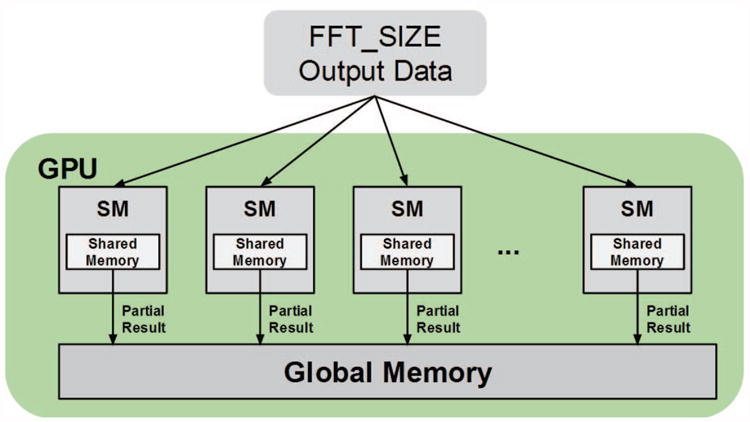
\includegraphics[width=0.6\linewidth]{piperKernel1}}
  \caption{Esquema para o primeiro kernel introduzido na versão GPU2014 \cite{piper2014gpu}. }
  \label{k1piper}
\end{figure}
 %kernel 2
% The second kernel uses only a single block. The number of threads in this block is equal to
%the number of blocks used in stage 1
% At each step, the number of active threads is equal to half the number of 
%partial scores remaining. Each thread compares two scores and writes the best to the lower
%half of memory. After every comparison, a synchronization is performed to ensure all
%threads are always operating on the same step and thus operating on the consistently updated
%memory. Eventually this results in a single top score. This best score is then marked in a
%separate array in global memory, indicating that it is a top score
%Along with
%marking the top score, positions in the molecular grid around this best score are also marked
%as being “top scores.”
 O kernel anterior usa mais do que um thread block, por sua vez o segundo \textit{kernel} apenas usa um bloco de threads (figura \ref{k2piper}). O bloco a usar tem de ter o mesmo número de threads que o número de blocos que foram usados no passo anterior. Cada uma das threads do bloco compara dois scores e escreve o melhor dos dois na memória partilhada para o bloco, sendo feita uma sincronização para garantir que as threads operam no mesmo passo de iteração e sobre memória consistente. O top score é determinado e guardado na memória global. \par
 \begin{figure}[ht]
  \centering
    {\includegraphics[width=0.6\linewidth]{piperKernel2}}
  \caption{Esquema para o segundo \textit{kernel} introduzido na versão GPU2014 \cite{piper2014gpu}. }
  \label{k2piper}
\end{figure}
 %Optimizações ocupação
% The second major optimization is the elimination of the idle GPU time when the rotation and
%grid assignment steps are performed on the CPU. In the original version, CUDA streams
%were used in an attempt to overlap GPU work with grid assignment [16]. However, due to
%the result from filtering and scoring immediately being assigned to memory and moved
%around on the CPU, the GPU \textit{kernels} were forced to execute filtering and synchronize before
%the CPU could prepare for the next rotation.
%To solve both of these issues, we move all of the grid assignment arrays permanently to the
%GPU and perform grid assignment and ligand rotation directly on the GPU. There is then no
%need for transfers between the host system memory and GPU memory. For this to be
%feasible, the GPU must contain enough global memory for all of the input and output data.
Para além da adição dos dois \textit{kernels} referidos anteriormente, o tempo em que o GPU não desempenha funções enquanto que a rotação e atribuições na grelha estão a ser processados pelo CPU foi eliminado. A computação da grelha do ligando passa a ser desempenhada pelo GPU, deixando de necessidade de a transferir entre a memória do \textit{host} e a do GPU. Esta optimização tem como requisito um GPU com memória global suficiente para armazenar os arrays relacionados com as atribuições da grelha do ligando. \par
 No entanto houve optimizações da solução GPU09 que foram mantidas. Nas etapas em que a aplicação do FFT às grelhas é feita, a optimização original consistiu em aplicar a bibilioteca cuFFT à semelhança do que foi feito para o Megadock sobre os passos que envolvem FFT sobre as grelhas. As restantes etapas foram paralelizadas mapeando todo o processo para o GPU, novamente à semelhança da implementação para o Megadock.
    \begin{figure}[ht]
  \centering
    {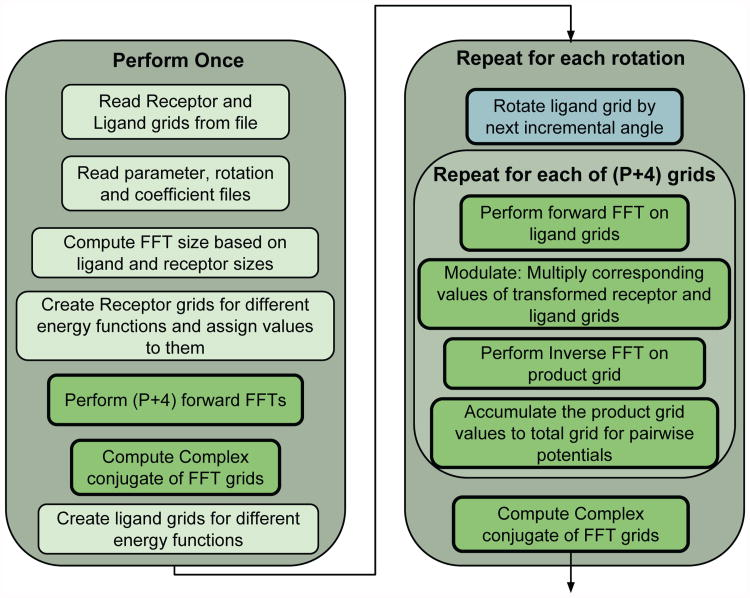
\includegraphics[width=0.6\linewidth]{piperFig}}
  \caption{Etapas do processo de docking no PIPER. As etapas destacadas a verde escuro foram aceleradas por GPU em 2009 e a etapa a azul em 2014. \cite{piper2014gpu} }
  \label{piperGPU}
\end{figure}

    \begin{figure}[ht]
  \centering
    {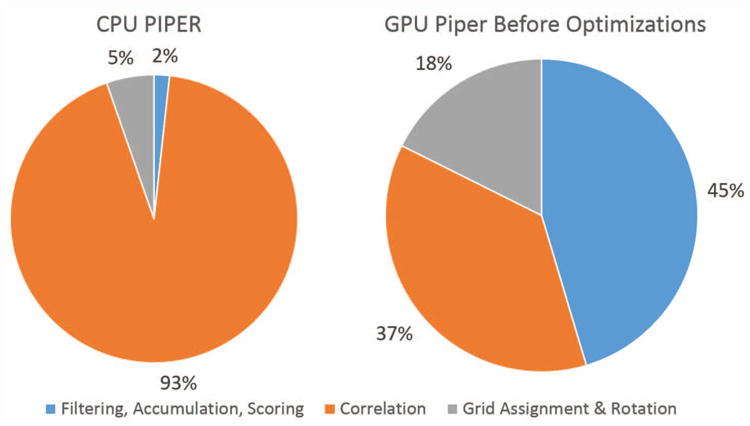
\includegraphics[width=0.6\linewidth]{cpuPoper}}
  \caption{Proporções de tempo gasto na execução para a versão CPU optimizada e a versão de 2009 que usa GPUs\cite{piper2014gpu} . }
  \label{propPiper}
\end{figure}
\subsubsection{Conclusões}
Esta subsecção mostra que nem sempre uma versão de um programa com acelerações em GPU é superior a uma outra versão mais recente do mesmo programa que use o CPU com optimizações. Pelo que é necessário adaptar o código às funcionalidades que as arquiteturas GPU correntes suportam assim como às alterações que o programa original sofre. As optimizações que foram aplicadas ao PIPER em 2014 foram aplicadas à fase de \textit{scoring}, mais precisamente às etapas de filtragem e cálculo dos \textit{scores} optimais. Pelo que é mostrado forma de optimizar a fase de \textit{scoring} do BiGGER, implementando uma redução como foi confirmado no caso do Megadock para a mesma etapa.
\subsection {AutoDock}
%introdução autodock
O AutoDock \cite{autoDock} é um programa diferente dos até agora indicados, não só por ser especifico para interações entre proteina-droga\footnote[10]{Uma droga é caracterizada  por uma molécula de pequenas dimensões.} como também por utilizar o algoritmo genético de Lamarck para determinar a posição correta dos elementos do par, em alternativa ao uso da complementaridade de superficie como função de score. Pelo que descarta as operações binárias que o BiGGER usa e as correlações usando FFT que os outros programas usam.
Actualmente, existem duas versões do software: AutoDock 4 e Vina\cite{autoDockVina}. O AutoDock 4 está dividido ainda em dois sub programas: \textit{autodock} faz o docking do ligando com um conjunto de grelhas que fazem a descrição do complexo resultante. O segundo, \textit{autogrid}, faz os cálculos prévios para obter as grelhas que o autodock necessita para desempenhar as suas funções.  
%Vantagens do Vina sobre o 4
O AutoDock Vina é diferente do AutoDock 4 no sentido de não efectuar o cálculo das grelhas de forma prévia mas sim instantaneamente, de forma automática, não guardando as grelhas em disco.
\subsubsection{Aceleração do AutoDock com o GPU}
%Introduzir informação sobre a implementação para GPU do autodock e em que medida é que pode ser utilizado para o BIGGER
 Em 2010 foi abordada, à semelhança do que foi feito para o Megadock assim como para o PIPER, uma possivel paralelização do AutoDock utilizando o GPU \cite{autodockCuda}. Neste caso a API utilizada foi o CUDA, sendo desenvolvida a versão 4.2.1 do AutoDock, que permite um speedup ao algoritmo genético que é utilizado, em 2 vezes, sendo este speedup semelhante ao do Vina sobre o AudoDock 4.  No entanto o Vina difere desta versão 4.2.1 no sentido de acelerar um algoritmo de pesquisa local que permite a redução das operações necessárias para chegar ao resultado final, enquanto que esta versão visa acelerar o algoritmo genético que o AutoDock utiliza para determinar a posição optimal do ligando encaixado com a proteina. Mais precisamente a função de fitness do algoritmo genético, que avalia a energia dos individuos da população constituida pelo algoritmo genético, sendo esta energia individual a soma da energia inter-molecular dos atomos do receptor e os do ligando.

Os autores deste projeto de aceleração do AutoDock consideraram duas opções: a primeira seria dedicar cada thread do GPU ao cálculo da energia total de um individuo ao que eles designaram  \textit{PerThread} e a segunda dedicar um bloco de threads do GPU para determinar essa energia total (\textit{PerBlock}). A primeira solução garante a saturação do GPU (taxa de ocupação alta) para milhares de individuos e a segunda oferece a mesma saturação para centenas de individuos.
A solução optada foi uma variante do \textit{PerBlock}, em que existem 5 \textit{kernels} de escrita/leitura para cada passo do algoritmo genético (inicialização de coordenadas atómicas do individuo, aplicar a torção até ao cálculo da energia interna) para as coordenandas atómicas respetivas a um individuo. De forma a eliminar a possibilidade de existir overhead, foi optado lançar um \textit{kernel} e guardar as coordenadas atómicas na memória partilhada. Por este factor, a solução foi renomeada para \textit{PerBlockCached}.
 %o que é que o BIGGER ganha com isto?
 \subsubsection{Conclusões}
 Foi demonstrado na subsecção \ref{megaD} uma possibilidade de solução para acelerar o BiGGER, em que é implementado um conjunto de \textit{kernels} para as diversas etapas, inclusive uma redução para determinar a solução optimal e mapeamentos de dados para o GPU. A solução para o AutoDock oferece uma forma de poder acelerar o cálculo da função de score do BiGGER utilizando a memória partilhada do GPU. 
 
 
 
% \subsection{Dinamica molecular em GPUs}
%Os programas a considerar nas proximas subsecções são o \textit{Chemistry at HARvard Macromolecular Mechanics} (CHARMM) e o \textit{Assisted Model Building with Energy Refinement} (AMBER) \cite{amber2013} não só por serem os mais utilizados pela comunidade, como também por serem os mais completos. Ambos têm um modelo de solvente implicito bem sucedido
%% Introdução 41
%%CHARMM at one extreme is a very complete modeling program that requires mastery of a fairly complex scripting language, but within which one can conduct a wide-variety of simulations and perform the widest variety of simulation analyses
%
%%UMa razao para so estarem estes dois aqui
%%The next crucial step in using all-atom molecular dynamics is to decide upon a solvent model; two typical choices are between a Generalized Born implicit solvent model (GB) and explicit solvent model. The second-generation of the GB models [24,25,26], which can be found in both CHARMM and AMBER, have shown great promise and application over the past several years [27-31], and are under active development [32,33]. These models have two key features: 1) the use of a semi-empirical potential which approximates the interaction between two charges within a protein (or more precisely two charges in a single dielectric material embedded within another dielectric) by extrapolating between two exact forms: the infinity-separated ion pair and the unified ion, and 2) approximating the Born radius, i.e., the energy of placing a single charge in a dielectric-embedded in water. \cite{salsbury2010molecular}
%\subsubsection{CHARMM}
%%250 palavras
%\subsubsection{AMBER}
%250 palavras
%O que ha para GPUs
% Desta implementação pode-se adaptar, caso seja necessário, a implementação de um \textit{kernel} para cada conjunto de etapas do BiGGER, desde a criação das grelhas até à atribuição dos valores binários core/surface, pode-se guardar as variáveis necessárias na memória partilhada do GPU. Esta adaptação poderá permitir reduzir a possibilidade de existir overhead na instanciação dos futuros \textit{kernels} do BIGGER.% A possibilidade de adaptar uma versão do \textit{PerBlockCached}
%% ====================
%% = Folder Structure =
%% ====================
%\section{Folder Structure} % (fold)
%\label{sec:folder_structure}
%
%The \novathesis\ template is organized into files and folders. At the main level it includes the following files and folders:
%
%\noindent
%\begin{tabularx}{\linewidth}{>{\ttfamily}l>{\itshape}l>{\upshape}X}
%novathesis.cls     & file    & 
%The main class file. It will include additional files from \texttt{novathesis-files} folder. 
%\\ 
%template.tex      & file    & 
%The main user file. Use this file as the main file for your thesis. 
%\\
%bibliography.bib  & file    & 
%An example of a bibliography file. You may have has many as you want. \\
%template.pdf      & file    & 
%A possible result of applying pdf\LaTeX\ to the \texttt{template.tex} file. The template supports multiple types of documents (e.g., MSc dissertation, PhD thesis, …) and multiple Schools (e.g., FCT-NOVA, FCSH-NOVA, IST-UL, FC-UL, …) and each will produce different results.
%\\
%Chapters          & folder  & Examples of thesis chapters. Replace them with your own chapters. 
%\\
%Examples          & folder  & Some more examples of the use of the template for different document types and Schools. 
%\\
%Scripts           & folder  & Some (possibly useful) scripts for Unix-based systems (Linux, Mac OSx). If you are a windows user, ignore this folder (you may safely delete it if you want). 
%\\
%novathesis-files   & folder  & 
%Additional files for the \novathesisclass\ file.  Unless you know what you are doing, avoid messing up with the files and folders inside this folder (except for deleting the unused Schools, see below). 
%\\
%\end{tabularx}
%
%The \texttt{novathesis-files} folder contains additional files and folders that complement the main \novathesisclass\ file.  These are:
%
%\noindent
%\begin{tabularx}{\linewidth}{>{\ttfamily}l>{\itshape}l>{\upshape}X}
%README.txt      & file    &
%A file that should be read!  :) 
%\\
%fix-babel.clo   & file    &
%Simple fixes to the \texttt{babel} package.
%\\
%lang-text.clo   & file    &
%Translations of important strings used in the template.  Currently fully supported are Portuguese and English, but French is on the way.  If you add translations for your own language, please be so kind and send them to me. Thank you!
%\\
%options.clo     & file    &
%Processing of \novathesisclass\ options.  \emph{Don't mess with this!}
%\\
%packages.clo    & file    &
%Additional packages to be loaded into the \novathesis\ template. \emph{You should not mess with this!}
%\\
%spine.clo       & file    &
%This file is loaded only if the option \texttt{spine=true}, and includes the typesetting of the book spine.
%\\
%ChapStyles      & folder  &
%Contains a lot of files, one for each chapter style.  If you really know what you are doing, you may add your own chapter style here.
%\\
%FontStyles      & folder  &
%Contains a few files, one for each set of fonts (main text font, chapter font, section font, subsection font, etc).  If you really know what you are doing, you may add your own set here.
%\\
%Schools         & folder  &
%Configuration files for each school.  This folder is organized into subfolders, one for each university.  \emph{You may safely delete all the subfolders except the one for your University.}  Then open the subfolder of your University and \emph{you may safely delete all the subfolders except the one for your School/Faculty}.
%\\
%\end{tabularx}
%
%As stated above, the \texttt{Schools} folder contains per-university folders and per-school (faculty) subfolders.  Currently these are the available folders:
%
%\noindent
%\begin{tabularx}{\linewidth}{>{\ttfamily}r@{~/~}>{\ttfamily}l>{\itshape}l>{\upshape}X}
%ul     & ist    & folder  & 
%The folder for the \href{http://www.tecnico.ulisboa.pt}{\emph{Instituto Superior Técnico}} of the \emph{University of Lisbon}.
%\\
%nova    & fcsh   & folder  & 
%The folder for the \href{http:www.fcsh.unl.pt}{\emph{Faculty of Human and Social Sciences}}  of the \emph{NOVA University of Lisbon}.
%\\
%nova    & fct    & folder  & 
%The folder for the \href{http:www.fct.unl.pt}{\emph{Faculty of Sciences and Technology}} of the \emph{NOVA University of Lisbon}.
%\\
%nova    & novaims    & folder  & 
%The folder for the \href{http:www.novaims.unl.pt}{\emph{Information and Management School}} of the \emph{NOVA University of Lisbon}.
%\\
%\end{tabularx}

%% section folder_structure (end)
%
%% ===================
%% = Package options =
%% ===================
%\section{\novathesisclass\ Class Options} % (fold)
%\label{sec:package_options}
%
%The \novathesis\ class can be customized with the options listed below.
%
%\newcommand{\classoption}[3]{\textbf{#1=OPT}\qquad #2\\\qquad\emph{#3}\\}
%
%\noindent
%\begin{ctabular}{@{}p{\linewidth}@{}}
%  \toprule
%  \classoption{docdegree}%
%    {phd(*), phdplan, phdprop, msc, mscplan, bsc}%
%    {The type of the document: PhD Thesis (default), PhD Plan, PhD Proposal, MSc Disseration, MSc Plan, BSc Report}
%    \midrule
%  \classoption{school}%
%		{nova/fct(*), nova/fcsh, nova/ims, ul/ist, ul/fc}%
%    {The name of the school. This option changes the typesetting of the cover and some School specific formating, like margins, fonts, paragraph spacing and indentation, etc…}
%    \midrule
%  \classoption{lang}%
%    {en(*), pt}%
%    {The main language for the document.  Currently only Portuguese and English are supported.  Other languages are expected to be support in forthcoming versions.}
%    \midrule
%  \classoption{fontstyle}%
%    {bookman, charter, fourier, kpfonts(*), mathpazo1, mathpazo2, newcent}%
%    {The font set to be used in the document.  Please note that a font set include definitions for the main text, headings, maths, etc.}
%    \midrule
%  \classoption{chapstyle}%
%    {bianchi, bluebox, brotherton, dash, default, elegant(*), ell, ger, hansen, ist, jenor, lyhne, madsen, pedersen, veelo, vz14, vz34, vz43}%
%    {The chapter style, i.e., the look of the chapter beginning.}
%    \midrule
%  \classoption{converlang}%
%    {en, pt(*)}%
%    {The language to be used when typesetting the cover page.}
%    \midrule
%  \classoption{otherlistsat}%
%    {front(*), back}%
%    {Where to put the other lists besides the table of contents. The default is (\texttt{front}) before the main text.  But some scientific areas prefer them at the end of the document (\texttt{back}), just before the Appendixes.}
%    \midrule
%  \classoption{aftercover}%
%    {true, false(*)}%
%    {Include or don't include the contents of the “\texttt{aftercover}” file. The default is for this file to be ignored (if if it exists).}
%    \midrule
%  \classoption{linkscolor}%
%    {darkblue(*), black}%
%    {The color for all the hyperlinks in the PDF file.  The “\texttt{media=paper}” option (see below) will override this option to “\texttt{black}”}
%    \midrule
%  \classoption{spine}%
%    {true, false(*)}%
%    {Generate the book spine and the last page in the PDF.}
%    \midrule
%  \classoption{biblatex}%
%    {OPT=\{list of options for \texttt{biblatex}\}}%
%    {Customize \texttt{biblatex}, the bibliography management system used in this class. Probably you will want to change the value of the \texttt{biblatex} “\texttt{style}” option. For other customizations of \texttt{biblatex} check its manual.}
%    \midrule
%  \classoption{memoir}%
%    {OPT=\{list of options for \texttt{memoir}\}}%
%    {Customize the base class \texttt{memoir}. The \texttt{memoir} manual should be the first document to be consulted when looking for “\textbf{how can I do this?}” You may wnat to change the base font size from 11pt to a smaller (10pt) or larger (12pt) size.  Also, remember to change the “\texttt{draft}” to final when your document is finished.}
%    \midrule
%  \classoption{media}%
%    {screen(*), paper}%
%    {Behavior to be customized in the school options/configuration. Expected definitions for screen are: left and right margins are equal and use colored links. Expected definitions for paper are: left and right margins are different and use black links.}
%    \bottomrule
%\end{ctabular}
%
%\section{Additional considerations about the class options} % (fold)
%\label{sec:additional_considerations}
%
%In this section we will provide some additional considerations about some of the customizations available as class options.
%
%\subsection{The main language} % (fold)
%\label{sub:the_main_language}
%
%The choice of the main language with the option “\texttt{lang=OPT}” affects:
%
%\begin{itemize}
%	\item \textbf{The order of the summaries.} First is printed the abstract in the main language and then in the foreign language. This means that if your main language for the document in English, you will see first the “abstract” (in English) and then the “resumo” (in Portuguese). If you switch the main language for the document for Portuguese, it will also automatically switch the order of the summaries to “resumo” and then “abstract”.
%	\item \textbf{The names for document sectioning.} E.g., ``Chapter'' vs.\ ``Capítulo'', ``Table of Contents'' vs.\ ``Índice'', ``Figure'' vs.\ ``Figura'', etc.
%	\item \textbf{The type of documents in the bibliogrpahy.} E.g., ``Technical Report'' vs.\ ``Relatório Técnico'', ``PhD Thesis'' vs.\ ``Tese de Doutoramento'', etc.
%\end{itemize} 
%
%No mater which language you chose, you will always have the appropriate hyphenation rules according to the language at that point. You always get Portuguese hyphenation rules in the ``Resumo'', english hyphenation rules in the ``Abstract'', and then the main language hyphenation rules for the rest of the document.
%
%% subsection the_main_language (end).
%
%% section additional_consideration (end)
%
%
%\subsection{Class of Text} % (fold)
%\label{sub:class_of_text}
%
%You must choose the class of text for the document. The available options are:
%
%\begin{enumerate}
%	\item \textbf{bsc} --- BSc graduation report.
%	\item \textbf{*mscplan} --- Preparation of MSc dissertation. This is a preliminary report graduate students at DI-FCT-NOVA must prepare to conclude the first semester of the two-semesters MSc work. The files specified by \verb!\dedicatoryfile! and \verb!\acknowledgmentsfile! are ignored, even if present, for this class of document.
%	\item \textbf{msc} --- MSc dissertation.
%	\item \textbf{phdprop} ---  Proposal for a PhD work. The files specified by \verb!\dedicatoryfile! and \verb!\acknowledgmentsfile! are ignored, even if present, for this class of document.
%	\item \textbf{prepphd} ---  Preparation of a PhD thesis. This is a preliminary report PhD students at DI-FCT-NOVA must prepare before the end of the third semester of PhD work. The files specified by \verb!\dedicatoryfile! and \verb!\acknowledgmentsfile! are ignored, even if present, for this class of document.
%	\item \textbf{phd} --- PhD dissertation.
%\end{enumerate}
%% subsection class_of_text (end)
%
%% ============
%% = Printing =
%% ============
%\subsection{Printing} % (fold)
%\label{sub:printing}
%
%You must choose how your document will be printed. The available options are:
%\begin{enumerate}
%	\item \textbf{oneside} --- Single side page printing.
%	\item \textbf{*twoside} --- Double sided page printing.
%\end{enumerate}
%% subsection printing (end)
%
%% =============
%% = Font Size =
%% =============
%\subsection{Font Size} % (fold)
%\label{ssec:font_size}
%
%You must select the encoding for your text. The available options are:
%\begin{enumerate}
%	\item \textbf{11pt} --- Eleven (11) points font size.
%	\item \textbf{*12pt} --- Twelve (12) points font size. You should really stick to 12pt\ldots
%\end{enumerate}
%% subsection font_size (end)
%
%% =================
%% = Text encoding =
%% =================
%\subsection{Text Encoding} % (fold)
%\label{ssec:text_encoding}
%
%You must choose the font size for your document. The available options are:
%\begin{enumerate}
%	\item \textbf{latin1} --- Use Latin-1 (\href{http://en.wikipedia.org/wiki/ISO/IEC_8859-1}{ISO 8859-1}) encoding.  Most probably you should use this option if you use Windows;
%	\item \textbf{utf8} --- Use \href{http://en.wikipedia.org/wiki/UTF-8}{UTF8} encoding.    Most probably you should use this option if you are not using Windows.
%\end{enumerate}
% subsection font_size (end)

% ============
% = Examples =
% ============
%\subsection{Examples} % (fold)
%\label{ssec:examples}
%
%Let's have a look at a couple of examples:
%
%\begin{itemize}
%	\item Preparation of PhD thesis, in portuguese, with 11pt size and to be printed single sided (I wonder why one would do this!)\\
%	\verb!\documentclass[prepphd,pt,11pt,oneside,latin1]{thesisdifct-nova}!
%	\item MSc dissertation, in english, with 12pt size and to be printed double sided\\
%	\verb!\documentclass[msc,en,12pt,twoside,utf8]{thesisdifct-nova}!
%\end{itemize}
%% subsection examples (end)
%
%\section{How to Write Using \LaTeX} % (fold)
%\label{sec:how_to_write_using_latex}
%
%Please have a look at Chapter~\ref{cha:a_short_latex_tutorial_with_examples}, where you may find many examples of \LaTeX constructs, such as Sectioning, inserting Figures and Tables, writing Equations, Theorems and algorithms, exhibit code listings, etc.
%
%% section how_to_write_using_latex (end)
%
%
%
%\section{Exmaple glossary and acronyms}
%%
%% \todo[inline]{A a note in a line by itself.}
%%
%This is the first occurrence of an abbreviation: \gls{abbrev}. And now the second occurrence of the same abbreviation: \gls{abbrev}. And a new acronym with capital letter: \Gls{xpt} and reused \gls{xpt}.  Let's also use a few other acronyms such as \gls{aaa}, \gls{aab}, \gls{aba}, \gls{bbb} and \gls{xpt}.
%
%
%Lets add the term ``\gls{computer}'' to the glossary!
%
% Please note that
% \begin{center}
%   \textbf{\large this package and template are not official for FCT/NOVA}.
% \end{center}
